% 黒魔術
\expandafter\ifx\csname ifdraft\endcsname\relax
    \documentclass[a4paper,twoside,12pt,papersize, dvipdfmx]{iirthesis}
    \usepackage{amsmath,amssymb,amsthm}
    \usepackage{graphicx}
    \usepackage{subcaption}
    \usepackage{url}
    \usepackage{otf}
    \usepackage{minitoc}
    \usepackage{bm}
    \usepackage{amsmath,amssymb}
    \usepackage{algorithm}
    \usepackage{algpseudocode}
    \begin{document}

    \newcommand{\figref}[1]{\figurename\ref{#1}}
    \newcommand{\tabref}[1]{\tablename\ref{#1}}
    \renewcommand{\eqref}[1]{式~(\ref{#1})}
    \newcommand{\chapref}[1]{\ref{#1}章}
    \newcommand{\secref}[1]{\ref{#1}節}
    \newcommand{\ssecref}[1]{\ref{#1}項}
    \newcommand{\appref}[1]{付録\ref{#1}}
    \newcommand{\algoref}[1]{Algorithm~\ref{#1}}
    
    \algnewcommand\algorithmicforeach{\textbf{for each}}
    \algdef{S}[FOR]{ForEach}[1]{\algorithmicforeach\ #1\ \algorithmicdo}
    \algnewcommand{\IIf}[1]{\State\algorithmicif\ #1\ \algorithmicthen}
    \renewcommand{\algorithmicrequire}{\textbf{Input:}}
    \renewcommand{\algorithmicensure}{\textbf{Output:}}
\fi

\newcommand{\tab}[0]{\;\;\;\;}

\chapter{ハンド動作計画の性能向上と新アルゴリズム}\label{chap::planner}
\minitoc

\section{はじめに}\label{sec::planner::intro}
%ハンドの寸法とかPCの性能の話,閾値,コンフィギュレーションの離散粗さ,動作計画で使ってる情報の説明
本章ではハンドの動作計画における先行研究からの改善点や新たな手法の提案を説明する.本節では,実際の動作計画に使用する設定情報についてまとめる.\par

\paragraph{ハンドの設定}
まずは,ハンドの設定についてである.ハンドは\ssecref{subsec::sicm::oppositehand}の対向型ハンドを以降の全ての動作計画に対して使用している.ハンドの寸法は以下のように設定した(\figref{fig::planner::handsize}).
\begin{gather}
\notag
\left\{
\begin{aligned}
L &= 60 \mathrm{[mm]} & w& = 35 \mathrm{[mm]} & h &= 415 \mathrm{[mm]}\\
d_0 &= 38 \mathrm{[mm]} & d_1 &= 130 \mathrm{[mm]} & d_2 &= 130 \mathrm{[mm]} & d_3 = 90 \mathrm{[mm]}
\end{aligned}
\right .
\end{gather}
ハンドの姿勢は,各関節角度$\theta_i$の集合$\bm {\theta}$により決定する.$\theta_i$は,この関節に連結している2リンクの内,根元側のリンクのリンク長方向を$0^\circ$とした時の手先側リンクのリンク長方向の角度と定義している.ここで,根元側リンクから見て,反時計回りを正としている.根元の関節に関しては,鉛直方向を$0^\circ$として定めている.
\begin{figure}[b]
\centering
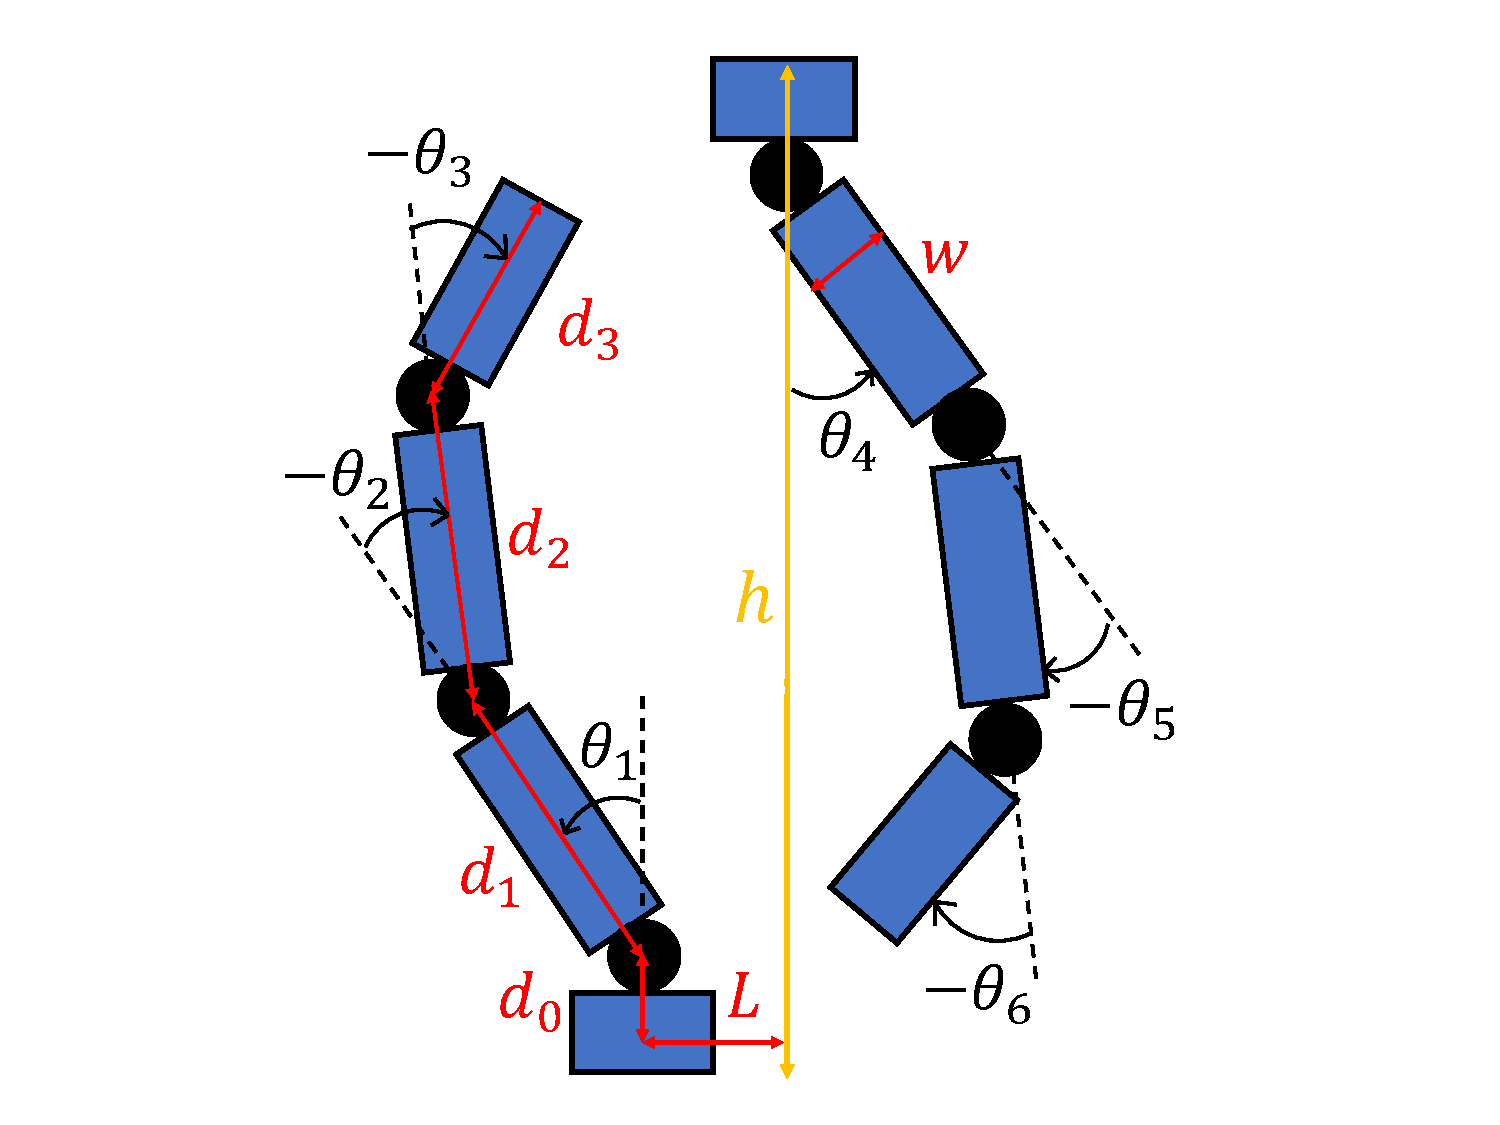
\includegraphics[width=0.7\hsize]{fig/3-new-planner/handsize.pdf}
\caption{Robot hand configuration}\label{fig::planner::handsize}
\end{figure}

\paragraph{対象物のコンフィギュレーション空間の設定}
対象物コンフィギュレーション空間は$-400 \mathrm{[mm]} \leq x \leq 400 \mathrm{[mm]}$,$-50 \mathrm{[mm]} \leq y \leq 550 \mathrm{[mm]}$,$0 \mathrm{[deg]} \leq \phi \leq 360 \mathrm{[deg]}$の直方体空間と設定した.$(x,y)$の原点は\figref{fig::planner::handsize}の原点$O$に相当し,$\phi$の原点は以下に記す対象物の姿勢$0^\circ$に相当する.前述の通り,コンフィギュレーション空間は格子状に分割し,離散的に取り扱っている.この格子点幅は$(\Delta x, \Delta y, \Delta \phi) = (10 \mathrm{[mm]}, 10 \mathrm{[mm]}, 5 \mathrm{[deg]})$と設定した.無限遠点$\mathcal{P}_{\mathrm {far}}$は以下の式で表される点群と設定した.なお,$C_{\mathrm {space}}$はコンフィギュレーション空間の全離散点群を表す.
\begin{gather}
\notag
\mathcal{P}_{\mathrm {far}} = \{ (x, y, \phi) \in C_{\mathrm {space}} \,|\, x = -400 \mathrm{[mm]} \lor x = 400 \mathrm{[mm]} \}
\end{gather}

\paragraph{対象物の形状情報}
本論文では,長方形物体,三角形物体,L字型物体,T字型物体を対象に動作計画を行った.これらの対象物の寸法情報や姿勢の定義について述べる.長方形物体は\figref{fig::planner::recdef}のように設定した.代表点は対角線の交点であり,姿勢は短辺が水平方向となるように置いた状態を$0^\circ$とした傾き角度となる.三角形物体は\figref{fig::planner::tridef}のように設定した.図心は外接円の中心であり,姿勢は$e_1$が水平方向となるように置いた状態を$0^\circ$とした傾き角度である.そのため,ユーザは三角形物体の形状情報を設定するとき,どの辺が$e_1$かを把握し,そのうえで目標姿勢を与える必要がある.L字型物体は\figref{fig::planner::lshapedef}のように設定した.図心は\figref{fig::planner::lshapedef}のように補助線を引いて得られる長方形の対角線交点である.姿勢は文字「L」を$0^\circ$とした傾き角度である.T字型物体は\figref{fig::planner::tshapedef}のように設定した.図心,姿勢ともにL字型と同様である.なお,傾きは$0 \mathrm{[deg]} \leq \phi \leq 360 \mathrm{[deg]}$で表し,反時計回りに測る.

\paragraph{PCのスペック}
OS:Ubuntu 22.04.1 LTS,CPU:AMD Ryzen 7 3700X 8-Core Processor,クロック周波数:4.43[GHz],RAM:32.0[GB]のPCで計算する.

\begin{figure}[b]
\centering
\begin{minipage}{0.49\hsize}
\centering
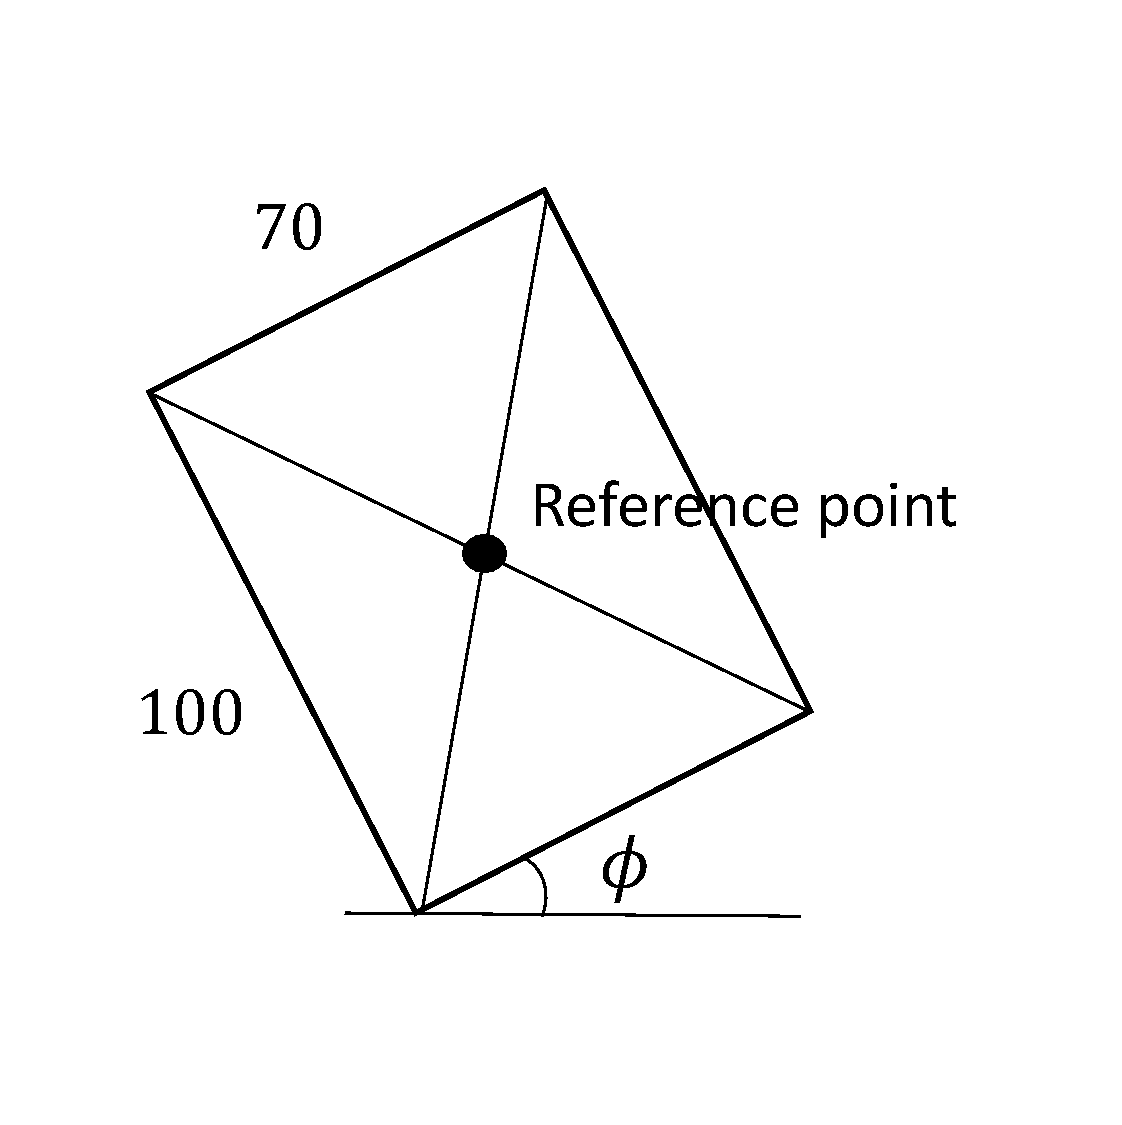
\includegraphics[width=0.9\hsize]{fig/3-new-planner/RectangleDef.pdf}
\caption{The definition of rectangle object}\label{fig::planner::recdef}
\end{minipage}\hfill
\begin{minipage}{0.49\hsize}
\centering
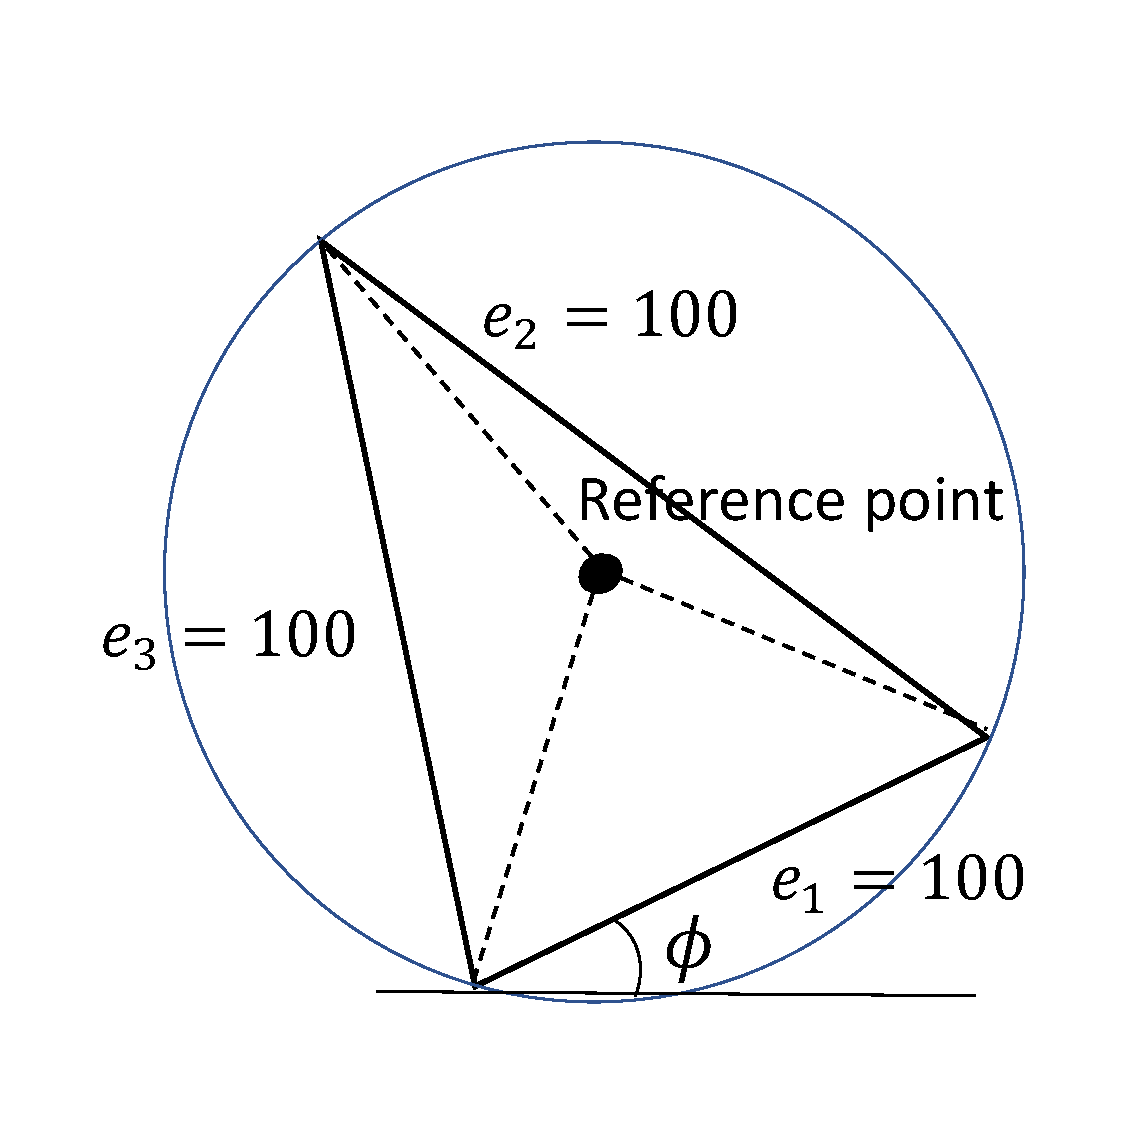
\includegraphics[width=0.9\hsize]{fig/3-new-planner/TriangleDef.pdf}
\caption{The definition of triangle object}\label{fig::planner::tridef}
\end{minipage}\hfill
\begin{minipage}{0.49\hsize}
\centering
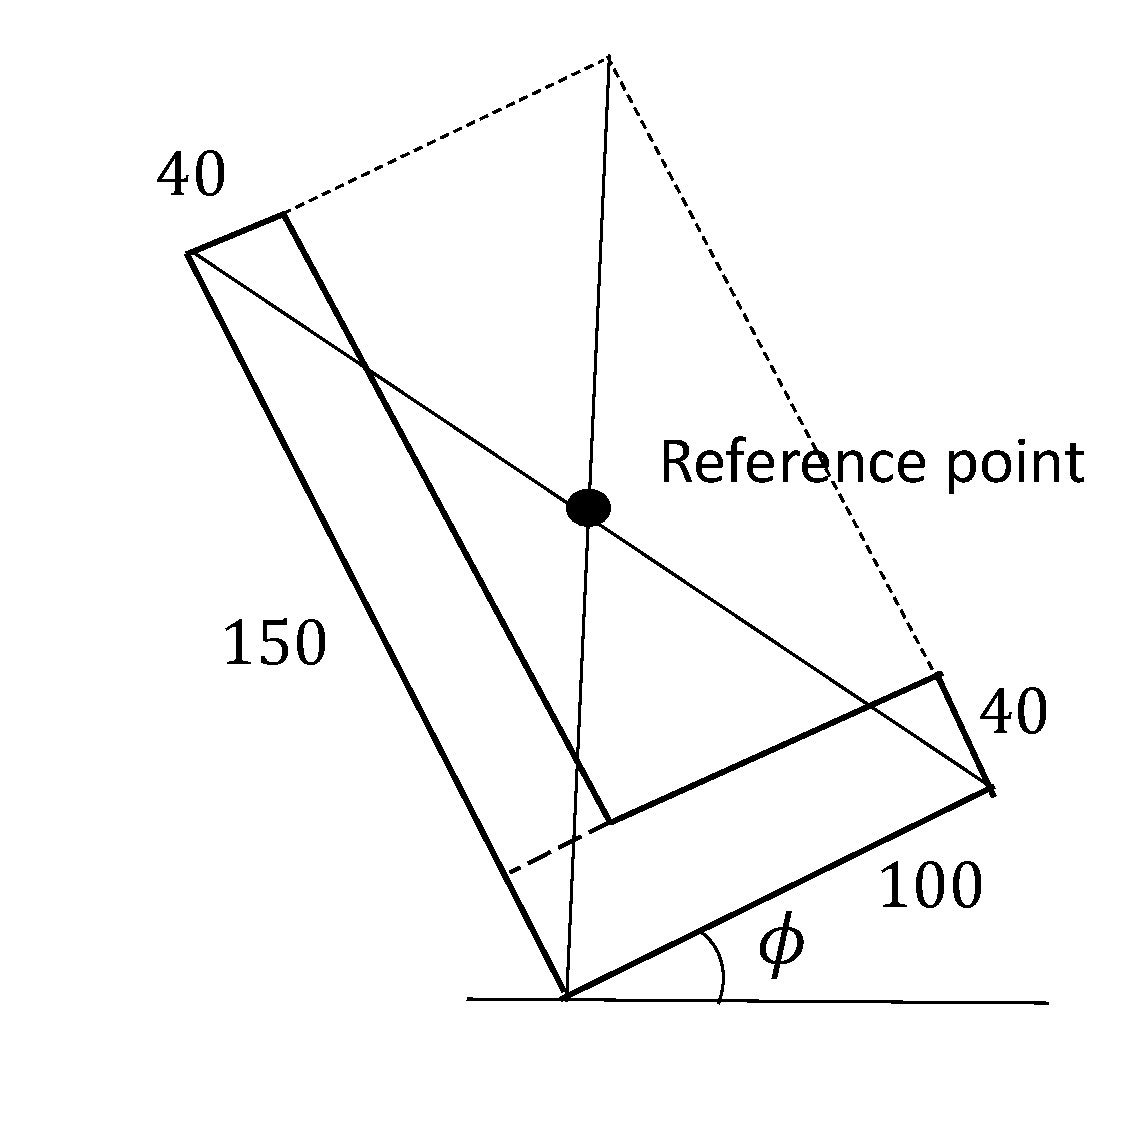
\includegraphics[width=0.9\hsize]{fig/3-new-planner/LShapeDef.pdf}
\caption{The definition of L-Shape object}\label{fig::planner::lshapedef}
\end{minipage}\hfill
\begin{minipage}{0.49\hsize}
\centering
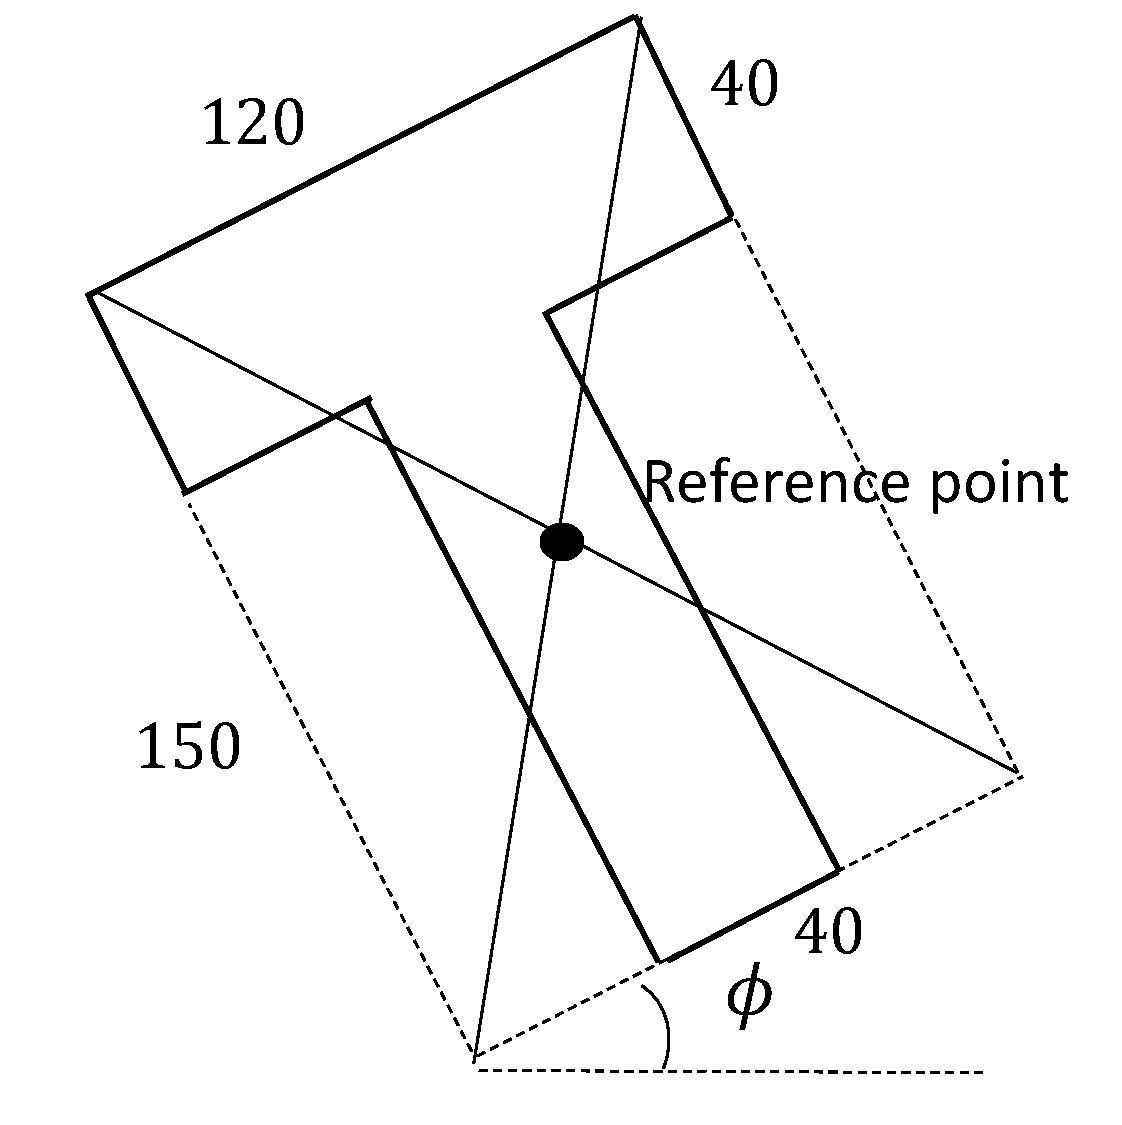
\includegraphics[width=0.9\hsize]{fig/3-new-planner/TShapeDef.pdf}
\caption{The definition of T-Shape object}\label{fig::planner::tshapedef}
\end{minipage}
\end{figure}

%%%%%%%%%%%%%%%%%%%%%%%%%%%%%%%%%%%%%%%%%%%%%%%%%%%%%%%%%%%%%%%%%%%%%%%%%%%%%%%%%%%%%%%%%%%%%%%%%%%%%%
%%%%%%%%%%%%%%%%%%%%%%%%%%%%%%%%%%%%%%%%%%%%%%%%%%%%%%%%%%%%%%%%%%%%%%%%%%%%%%%%%%%%%%%%%%%%%%%%%%%%%%
\section{順探索アルゴリズム}\label{sec::planner::straight}
改めて\chapref{chap::sicm}のハンド動作計画の流れを振り返る.まず,入力はハンドの初期姿勢と対象物の形状情報,そして対象物の目標位置・姿勢である.これらを基に,ハンド初期姿勢からRRTによりランダムにサンプリングし,その都度対象物の形状情報から$\mathcal{C}_{\mathrm{free\_obj}}$を計算する.ケージング成立条件,ケージングマニピュレーション可能条件の満足を確認しつつ探索を進め,対象物の目標位置・姿勢から決まる探索終了条件を満たせば動作計画が完了する.出力としては,ハンドの関節角度の時系列データが得られる.\par
この動作計画アルゴリズムを順探索アルゴリズムと呼ぶこととする.この順探索アルゴリズムには,計算時間が遅い,位置決め精度が悪いという2つの課題がある.以下の項は,これらの解決方法についてであり,前者の課題に対しては,\ssecref{subsec::planner::goalcond},\ssecref{subsec::planner::dfs}で,後者の課題に対しては,\ssecref{subsec::planner::formclosure}で説明する.

\subsection{探索終了条件の緩和}\label{subsec::planner::goalcond}
\secref{sec::sicm::planning}の通り,先行研究では対象物の目標位置・姿勢として$P_G (x_{\mathrm {goal}}, y_{\mathrm {goal}}, \phi_{\mathrm {goal}})$のコンフィギュレーション空間の1点を指定していた.しかし,本手法はパーツフィーダへの応用を想定しており,この際対象物を整列後,ベルトコンベアに乗せて生産ライン方向である$x$方向へ流す.そのため,$x$方向への目標設定は必須ではない.そこで,対象物の目標位置・姿勢を$P_G (x_{\mathrm {any}}, y_{\mathrm {goal}}, \phi_{\mathrm {goal}})$と$y$,$\phi$のみを指定するようにした.\par
これに従って,収束度$e$の定義を\eqref{eq::planner::e}のように変更した.
\begin{gather}
\begin{aligned}
&e = \max \sqrt{(w_1\Delta x)^2 + (w_2(y-y_{\mathrm{goal}}))^2 + (w_3(\phi-\phi_{\mathrm{goal}}))^2} \label{eq::planner::e} \\
%e \leq \varepsilon \label{eq::planner::goalcondition} \\
&ここで,\tab
 \Delta x = \dfrac{\max x  - \min x}{2} ,\;\; (x, y, \phi) \in \mathcal{C}_{\mathrm{free\_obj}}
\end{aligned}
\end{gather}
これにより,$x$方向に関しては座標の調整が必要なくなったため,先行研究より早い探索終了が見込める.

\subsubsection{計算時間の比較}
探索終了条件の緩和により計算時間に差が出るか検証する.なお,従来の探索終了条件を用いたものは基本的に\cite{komiyama2021}で用いていたアルゴリズムと同様であるが,プログラミング言語をPythonからC++に書き換え,処理を一部効率化することで約10倍程度,速度が改善したものとなっている.\par
L字形物体を用いて以下のように問題設定した.
\begin{gather}
\left\{
\notag
\begin{aligned}
&ハンド初期姿勢:[55, -55, -47, -6, 52, -47]\mathrm{[deg]}\\
&対象物の目標位置・姿勢:[x_{\mathrm {goal}}, y_{\mathrm {goal}}, \phi_{\mathrm {goal}}] = [{\mathrm {any}}, 200 \mathrm{[mm]}, 0 \mathrm{[deg]}]\\
&対象物:\mathrm{L}字形物体\\
&順探索の終了閾値:\varepsilon = 50\\
\end{aligned}
\right .
\end{gather}

ここで,探索終了条件を考える際,\eqref{eq::planner::e}の収束度$e$の定数$w_1$,$w_2$,$w_3$を次のように設定した.
\begin{gather}
\notag
w_1=1 \mathrm{[mm^{-1}]} \tab w_2=1 \mathrm{[mm^{-1}]} \tab w_3=1 \mathrm{[deg^{-1}]}
\end{gather}
以降の収束度$e$の計算にもこれらの値を用いる.\par

10回動作計画を行い,計算時間を測定した.結果を\tabref{tab::planner::goalconddiff},\figref{fig::planner::goalconddiff}に示す.
\begin{table}[bt]
    \centering
    \caption{Comparison of calculation time between previous goal condition and relieved goal condition}
    \label{tab::planner::goalconddiff}
    \begin{tabular}{c|r r}
        ~ & Previous goal [s] & Releived goal [s]  \\ \hline
        1 & 9412.5 & 1686.1  \\ 
        2 & 6322.1 & 800.2 \\ 
        3 & 1059.8 & 543.8  \\ 
        4 & 2364.4 & 822.6  \\ 
        5 & 429.5 & 743.8 \\ 
        6 & 819.4 & 366.4  \\ 
        7 & 2960.0 & 1816.2  \\
        8 & 610.5 & 130.3  \\ 
        9 & 1151.3 & 899.4  \\ 
        10 & 756.6 & 593.2  \\ \hline
        Average & 2588.6  & 840.2  \\ \hline
        SD & 2984.3 & 533.3  \\ 
    \end{tabular}
\end{table}
\begin{figure}[bt]
\centering
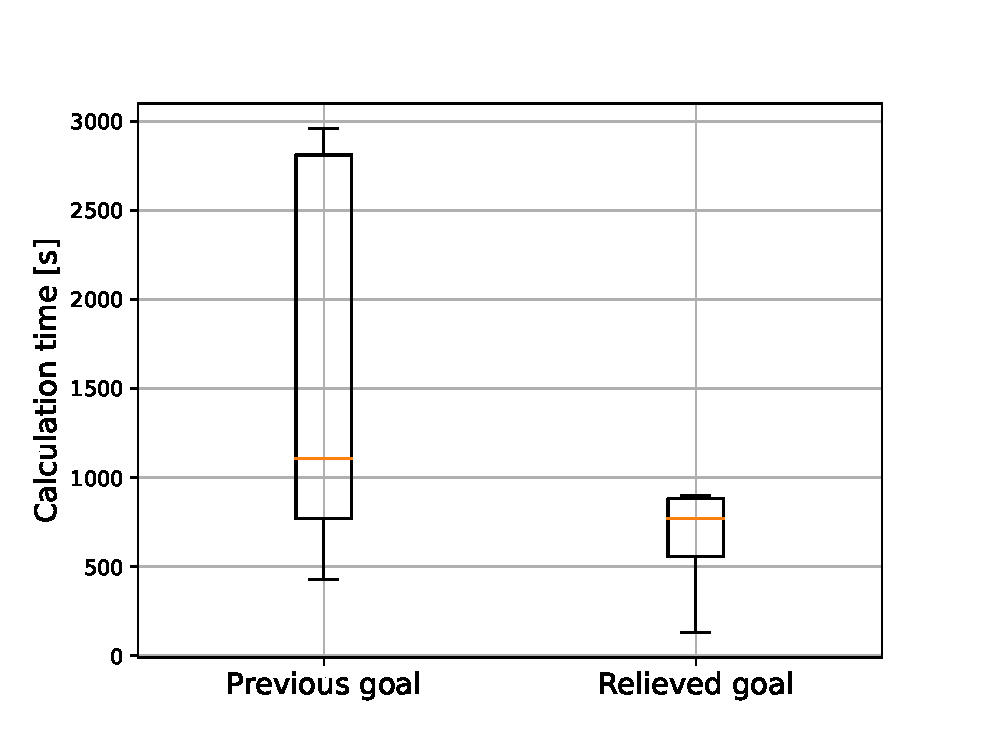
\includegraphics[width=0.5\hsize]{fig/3-new-planner/3_2_1.eps}
\caption{The box plot comparing calculation time between previous goal condition and relieved goal condition}
\label{fig::planner::goalconddiff}
\end{figure}

まず,2つのデータが等分散か否かを$F$検定により判断する.有意水準$5\%$とし,両側検定を行う.
\begin{gather}
\left\{
\notag
\begin{aligned}
&帰無仮説& &H_0:\sigma_1^2 = \sigma_2^2\\
&対立仮説& &H_1:\sigma_1^2 \neq \sigma_2^2\\
&検定統計量& &T = \dfrac{s_1^2}{s_2^2} = 31.3\\
&棄却域& &F(f_1, f_2; \alpha/2)=F(9, 9; 0.025) = 4.026\\
\end{aligned}
\right .
\end{gather}
$T=31.3 > 4.026$なので,$H_0$は棄却され,2つのデータは等分散ではないといえる.\par
2つのデータは非等分散なので,ウェルチの$t$検定により両側探索アルゴリズムの平均計算時間が順探索アルゴリズムに比べて有意に短いことを示す.
有意水準を$5\%$とし,片側検定を行う.
\begin{gather}
\left\{
\notag
\begin{aligned}
&帰無仮説& &H_0:\mu_1 = \mu_2\\
&対立仮説& &H_1:\mu_1 \geq \mu_2\\
&検定統計量& &T = \dfrac{\overline{x}_{1}-\overline{x}_{2}}{\sqrt{\dfrac{s_1^{2}}{n_{1}}+\dfrac{s_2^{2}}{n_{2}}}} = 1.82\\
&自由度& &f=\dfrac{1}{\dfrac{C^2}{n_1-1}+\dfrac{(1-C)^2}{n_2-1}}=9.57 \simeq 10 & \because C=\dfrac{\dfrac{s_1^2}{n_1}}{\dfrac{s_1^2}{n_1}+\dfrac{s_2^2}{n_2}}\\
&棄却域& &t(f, \alpha/2) = t(10, 0.05) = 1.81
\end{aligned}
\right .
\end{gather}
$T=1.82 > 1.81$なので,$H_0$は棄却され,探索終了条件の緩和により計算時間が有意に短くなることが示された.


\subsection{$\mathcal{C}_{\mathrm{free\_obj}}$の効率的な抽出}\label{subsec::planner::dfs}
\cite{komiyama2021}では$\mathcal{C}_{\mathrm{free\_obj}}$の抽出にあたって以下のような方法が取られていた.
\begin{enumerate}
\item 対象物のコンフィギュレーション空間の離散点群を全走査し,$\mathcal{C}_{\mathrm{free}}$を取り出す \label{planner::fullscan}
\item DBSCAN法\cite{ester1996}により隣り合う周囲26点群を同クラスタとするクラスタリングを$\mathcal{C}_{\mathrm{free}}$に対して行う\label{planner::clustering}
\item 手順\ref{planner::clustering}のクラスタを$\mathcal{C}_{\mathrm{free\_ICS}}$と$\mathcal{C}_{\mathrm{free\_ECS}}$に分ける
\item $\mathcal{C}_{\mathrm{free\_ICS}}$の内,\eqref{eq::sicm::continuous}に基づいて$\mathcal{C}_{\mathrm{free\_obj}}$を抽出する
\end{enumerate}
対象物のコンフィギュレーション空間の離散粗さを\secref{sec::planner::intro}のように設定した場合,点群数は約33万個となる.手順\ref{planner::fullscan}では,この点群を全走査するため計算時間が長くかかり,ボトルネックとなっている.\par

そこで,\eqref{eq::sicm::continuous}の直前$(t-\Delta t)$のハンド姿勢における$\mathcal{C}_{\mathrm{free\_obj}}(t-\Delta t)$と現在$(t)$のハンド姿勢における$\mathcal{C}_{\mathrm{free\_obj}}(t)$はオーバーラップしているという性質を応用して,$\mathcal{C}_{\mathrm{free\_obj}}(t-\Delta t)$を起点として,オーバーラップしている$\mathcal{C}_{\mathrm{free\_ICS}}$を直接探すという手法を提案する.\par

まず,$\mathcal{C}_{\mathrm{free\_obj}}(t-\Delta t)$の任意の一点を取り出す.壁やロボットハンドとの干渉がないか確認し,干渉があった場合は別の点を取り出す.この点を起点として周囲を探索し,この点が属する領域の境界線を見つけることで領域を取り出す.このとき,\figref{fig::planner::numbering}のように周囲の26個の方向に番号を付け,\figref{fig::planner::treegraph}のような木構造を作成する.この木構造は,根が取り出した起点,節,葉が起点周囲の点群となっており,周囲の探索手順の全組み合わせを表している.例えば根から1,2,5と進んだ場合は,起点から1の方向の点へ移動し,続いてそこを中心と考えたときの2の方向へ進み,さらに5の方向へ3ステップ進んだ点へ到達していることを表す.\par

この木構造を用いて,「深さ優先」のアプローチで探索を行う.
もし,探索が$\mathcal{P}_{\mathrm {far}}$へ到達した場合,つまり探索中の領域の境界線が見つからず,$\mathcal{C}_{\mathrm{free\_ECS}}$であった場合,その領域は破棄することとなる.無駄な探索を増やさないため,その領域が$\mathcal{P}_{\mathrm {far}}$へ到達するかどうかはなるべく早く判断したい.幅優先探索のようなアプローチを取ると,起点から全方向へ同じペースで探索が進むため,$P_{\mathrm {far}}$への到達が遅くなり,無駄な探索が多くなる.そこで,深さ優先探索というアプローチを取ると,任意の方向へ一直線に進めるだけ進むため,早い段階で$\mathcal{P}_{\mathrm {far}}$へ到達することができる.\par

\begin{figure}[bt]
\centering
\begin{minipage}{0.4\hsize}
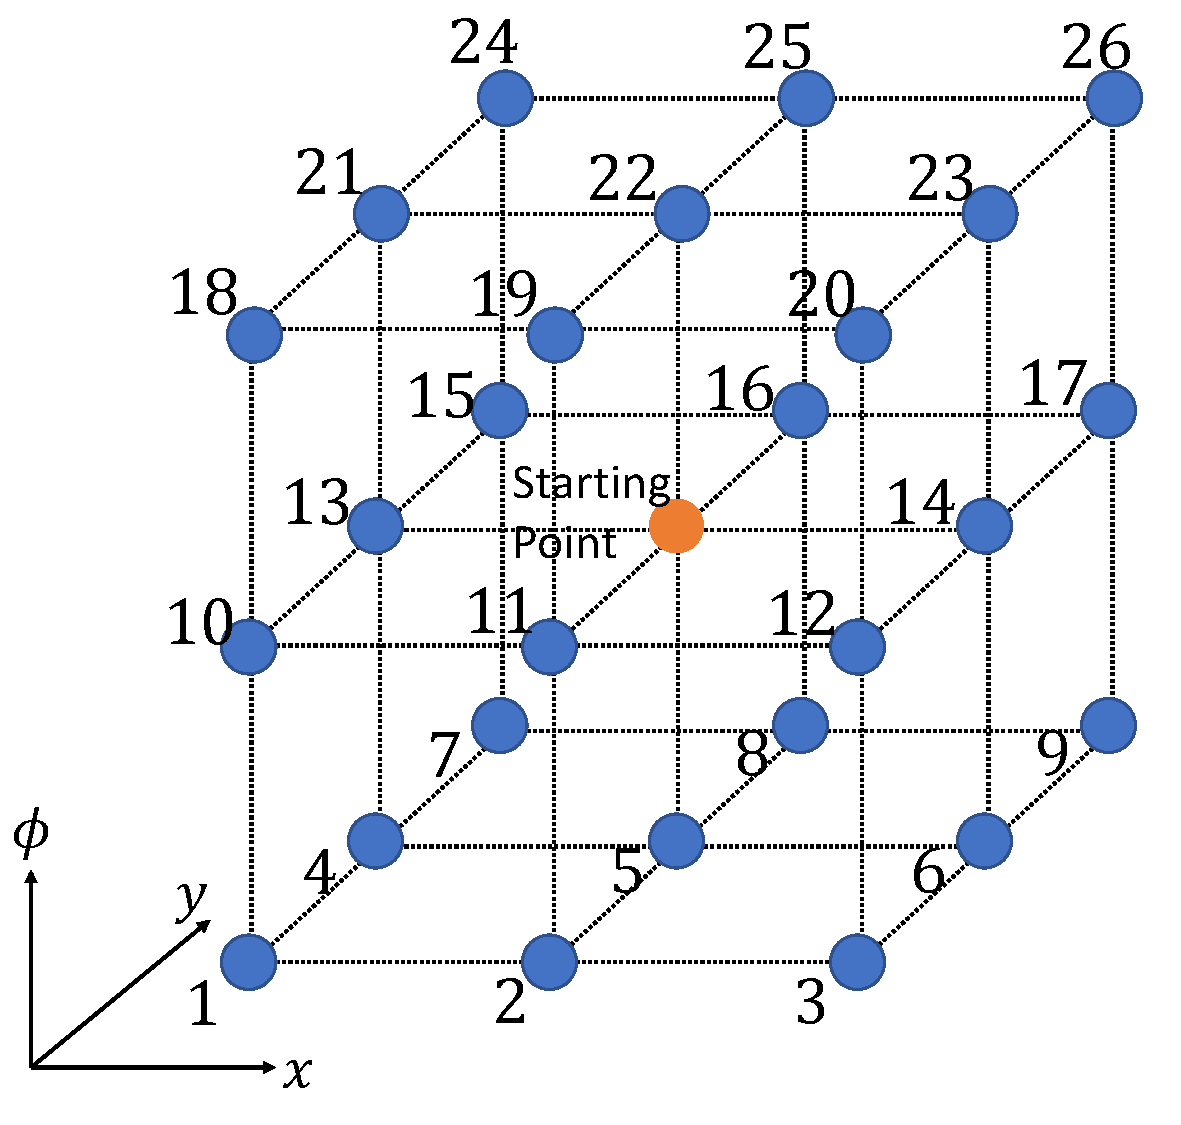
\includegraphics[width=0.9\hsize]{fig/3-new-planner/directiondef.pdf}
\caption{The definition of numbering}\label{fig::planner::numbering}
\end{minipage}\hfill
\begin{minipage}{0.59\hsize}
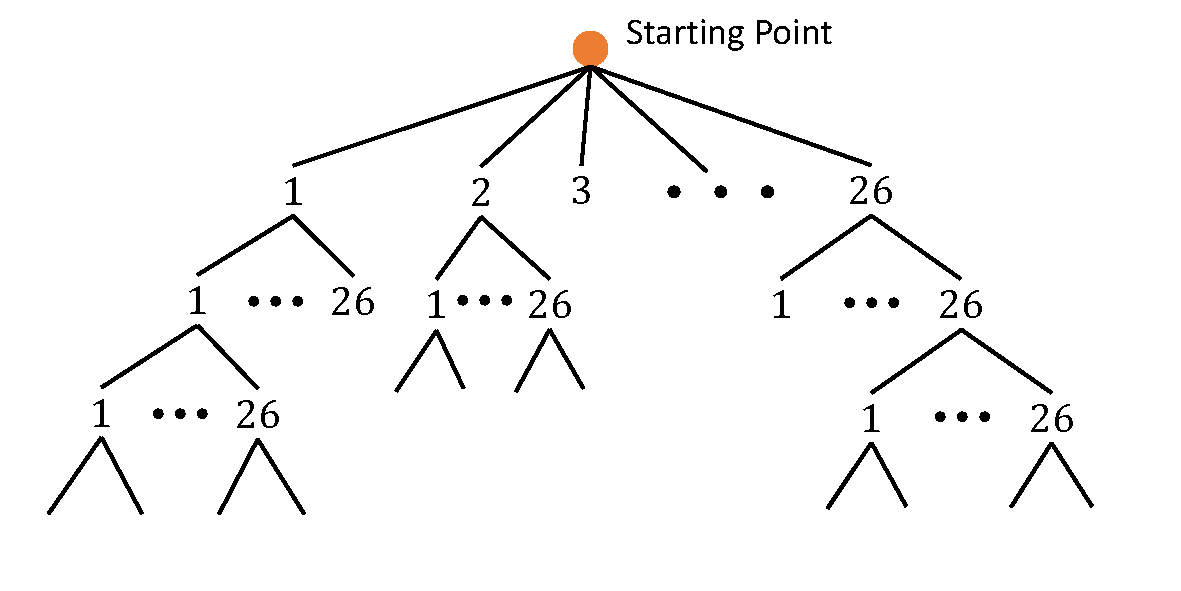
\includegraphics[width=\hsize]{fig/3-new-planner/treegraph.pdf}
\caption{Generating tree structure}\label{fig::planner::treegraph}
\end{minipage}
\end{figure}

以上より,木構造を深さ優先探索していく.探索中に壁やロボットハンドとの干渉があり,$\mathcal{C}_{\mathrm{free}}$でない点が現れたときは,その点が探索中の領域の境界線となる.その点より先の探索,つまり葉側の探索は注目領域外であり,不必要なので行わない.木構造の全ての探索が終わり,$\mathcal{P}_{\mathrm {far}}$へ到達しなかった場合,$\mathcal{C}_{\mathrm{free\_obj}}(t)$として認められる.\par

上記の一連の処理後,$\mathcal{C}_{\mathrm{free\_obj}}(t-\Delta t)$の内,探索されていない点がある場合を考える.この点は上で探索された領域外の点を意味し,この点が属する領域も$\mathcal{C}_{\mathrm{free\_obj}}(t)$になりうる.そのため,この点を起点とした探索を再度行う.\par

これを,$\mathcal{C}_{\mathrm{free\_obj}}(t-\Delta t)$の全ての点が探索されるまで行うことで過不足ない$\mathcal{C}_{\mathrm{free\_obj}}(t)$が抽出される.以上のアルゴリズムをより具体的にまとめたものを\algoref{algo::planner::dfs}に示す.なお,\algoref{algo::planner::dfs}では処理を関数にまとめ一般化しており,各々$(t-\Delta t)$はpreviousに,$t$はcurrentに該当する.

\begin{algorithm}[tb]
\caption{Efficient extraction of $\mathcal{C}_{\mathrm{free\_obj}}$}
\label{algo::planner::dfs}
\begin{algorithmic}[1]
\Function{efficient\_extraction}{$\mathcal{C}_{\mathrm{free\_obj}}(\mathrm {previous})$, Robot hand posture $\bm{\theta}$}
\State{$\mathcal{C}_{\mathrm{free\_obj}}(\mathrm {current}) \leftarrow \mathrm{empty}$}
\State{$\mathcal{C}_{\mathrm{delete}} \leftarrow \mathrm{empty}$}
\State{Update the robot hand posture to $\bm{\theta}$}
\ForEach{$\mathrm{Coordinate} \; p \in \mathcal{C}_{\mathrm{free\_obj}}(\mathrm {previous})$}	\label{forbegin}
\State{$\mathcal{C}_{\mathrm{candidate}} \leftarrow \mathrm{empty}$}
\IIf{$p$ has been explored} \textbf{continue}
\IIf{\Call{validation}{$p$} is `false'} \textbf{continue}
\State{$\mathcal{C}_{\mathrm{candidate}} \xleftarrow{\mathrm{add}} p$}
\State{$\mathrm{stack} \xleftarrow{\mathrm{push}} p$}

\While{stack size $\neq 0$}
\State{$q \xleftarrow{\mathrm{pop}} \mathrm{stack}$}
\For{$ i \leftarrow 1, 26$}
\State{Move $q$ to direction `$i$'}
\If{$q$ is a part of $\mathcal{P}_{\mathrm {far}}$ \textbf{or} 
       $q$ is a part of $\mathcal{C}_{\mathrm{delete}}$}
\State{$\mathcal{C}_{\mathrm{delete}} \xleftarrow{\mathrm{add}} \mathcal{C}_{\mathrm{candidate}}$}
\State{\textbf{goto} line \ref{forbegin}}
\EndIf
\IIf{\Call{validation}{$p$} is `false'} \textbf{continue}
\State{$\mathcal{C}_{\mathrm{candidate}} \xleftarrow{\mathrm{add}} q$}
\State{$\mathrm{stack} \xleftarrow{\mathrm{push}} q$}
\EndFor
\EndWhile
\State{$\mathcal{C}_{\mathrm{free\_obj}}(\mathrm {current}) \xleftarrow{\mathrm{add}} \mathcal{C}_{\mathrm{candidate}}$}
\EndFor
\State{\textbf{return} $\mathcal{C}_{\mathrm{free\_obj}}(\mathrm {current})$}
\EndFunction
\\

\Function{validation}{$\mathrm{Coordinate} \; c$}
\State{Update the position and orientation of the object to `c'}
\IIf{The object intersects with the robot hand} \textbf{return} false
\IIf{The object intersects with the wall} \textbf{return} false
\State{\textbf{return} true}
\EndFunction

\end{algorithmic}
\end{algorithm}

\clearpage

\subsubsection{計算時間の比較}
\begin{figure}[b]
\centering
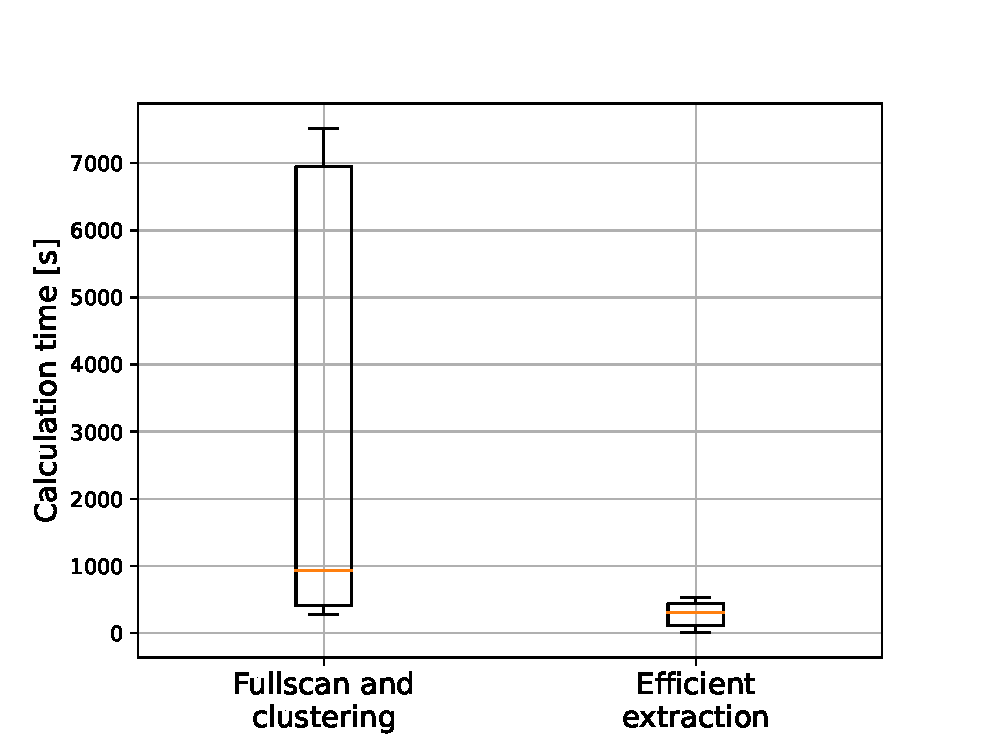
\includegraphics[width=0.5\hsize]{fig/3-new-planner/3_2_2.eps}
\caption{The box plot comparing calculation time between full scan and clustering extraction and efficient extraction of $\mathcal{C}_{\mathrm{free\_obj}}$}
\label{fig::planner::rasterdfs}
\end{figure}

$\mathcal{C}_{\mathrm{free\_obj}}$の効率的な抽出によって,計算時間に有意な差があるかを判定する.
三角形物体に対して,以下のように問題を設定した.ここで,通常コンフィギュレーション空間の姿勢$\phi$方向の幅は\secref{sec::planner::intro}の通り,$0 \mathrm{[deg]} \leq \phi \leq 360 \mathrm{[deg]}$で設定している.しかし,三角形物体は$120^\circ$で回転対称となっており,$0 \mathrm{[deg]} \leq \phi \leq 120 \mathrm{[deg]}$で全ての姿勢を表せる.コンフィギュレーション空間の幅が狭まると,離散点群数も減り計算負荷が軽くなるため,本動作計画ではこの$\phi$幅で計算する.以降,$\phi$幅を狭めた場合は記述するが,記述がない場合は$0 \mathrm{[deg]} \leq \phi \leq 360 \mathrm{[deg]}$で計算するものとする.
\begin{gather}
\left\{
\notag
\begin{aligned}
&ハンド初期姿勢:[34, -45, -30, 34, -45, -30]\mathrm{[deg]}\\
&対象物の目標位置・姿勢:[x_{\mathrm {goal}}, y_{\mathrm {goal}}, \phi_{\mathrm {goal}}] = [{\mathrm {any}}, 200 \mathrm{[mm]}, 0 \mathrm{[deg]}]\\
&対象物:三角形物体\\
&順探索の終了閾値:\varepsilon = 50\\
&コンフィギュレーション空間の\phi の範囲:0 \leq \phi \leq 120 \mathrm{[deg]}
\end{aligned}
\right .
\end{gather}

10回動作計画を行い,計算時間を測定した.結果を\tabref{tab::planner::rasterdfs},\figref{fig::planner::rasterdfs}に示す.
\begin{table}[b]
    \centering
    \caption{Comparison of calculation time between full scan and clustering extraction and efficient extraction of $\mathcal{C}_{\mathrm{free\_obj}}$}
    \label{tab::planner::rasterdfs}
    \begin{tabular}{c|r r}
        ~ & 
        \begin{tabular}{c}
        Full scan and \\clustering [s] 
        \end{tabular}
        &
        \begin{tabular}{c}
        Efficient \\extraction [s] 
        \end{tabular}
        \\ \hline
        1 & 7516.1 & 353.5 \\ 
        2 & 640.6 & 527.7  \\ 
        3 & 493.0 & 252.1    \\ 
        4 & 21322.8 & 135.0    \\ 
        5 & 294.4 & 461.2   \\ 
        6 & 274.4 & 65.4    \\ 
        7 & 390.5 & 202.7   \\ 
        8 & 26870.2 &140.9   \\
        9 & 5225.8 &1276.1  \\
        10 & 1213.7 &  389.0  \\ \hline
        Average & 6424.2 & 357.1  \\ \hline
        SD & 9719.5 &  367.9  \\
    \end{tabular}
\end{table}

まず,2つのデータが等分散か否かを$F$検定により判断する.有意水準$5\%$とし,両側検定を行う.
\begin{gather}
\left\{
\notag
\begin{aligned}
&帰無仮説& &H_0:\sigma_1^2 = \sigma_2^2\\
&対立仮説& &H_1:\sigma_1^2 \neq \sigma_2^2\\
&検定統計量& &T = \dfrac{s_1^2}{s_2^2} = 698.0\\
&棄却域& &F(f_1, f_2; \alpha/2)=F(9, 9; 0.025) = 4.026\\
\end{aligned}
\right .
\end{gather}
$T= 698.0 > 4.026$なので,$H_0$は棄却され,2つのデータは等分散ではないといえる.\par
2つのデータは非等分散なので,ウェルチの$t$検定により両側探索アルゴリズムの平均計算時間が順探索アルゴリズムに比べて有意に短いことを示す.
有意水準を$5\%$とし,片側検定を行う.
\begin{gather}
\left\{
\notag
\begin{aligned}
&帰無仮説& &H_0:\mu_1 = \mu_2\\
&対立仮説& &H_1:\mu_1 \geq \mu_2\\
&検定統計量& &T = \dfrac{\overline{x}_{1}-\overline{x}_{2}}{\sqrt{\dfrac{s_1^{2}}{n_{1}}+\dfrac{s_2^{2}}{n_{2}}}} = 1.97\\
&自由度& &f=\dfrac{1}{\dfrac{C^2}{n_1-1}+\dfrac{(1-C)^2}{n_2-1}}= 9.03 \simeq 9 & \because C=\dfrac{\dfrac{s_1^2}{n_1}}{\dfrac{s_1^2}{n_1}+\dfrac{s_2^2}{n_2}}\\
&棄却域& &t(f, \alpha/2) = t(9, 0.05) = 1.83
\end{aligned}
\right .
\end{gather}
$T= 1.97 > 1.83$なので,$H_0$は棄却され,探索終了条件の緩和により計算時間が有意に短くなることが示された.

\subsection{位置決め精度向上アルゴリズム}\label{subsec::planner::formclosure}
計算時間の観点から,収束度$e$は広めに設定したい.この場合,動作計画で得られたハンド最終姿勢では対象物の位置・姿勢決め精度は十分ではなくなる.そこで,以降に示す方法によって動作計画で得られたハンド最終姿勢から微調整を加え,位置決め精度の向上を試みた.
\subsubsection{アルゴリズム}
本アルゴリズムでは,動作計画により得られた最終姿勢から更に狭まる方向へ,更にケージングが強まる方向へ微調整する.そのため,この微調整中はケージング成立条件,ケージングマニピュレーション可能条件の両者が成立していると考え,本アルゴリズムではこれを前提としている.以下,具体的なアルゴリズムについて述べる.\par
まず,対象物を目標位置・姿勢$P_G (x_{\mathrm m}, y_G, \theta_G)$に仮想的に配置する.ここで,$x$座標の目標位置$x_{\mathrm m}$に関して,\ssecref{subsec::planner::goalcond}の方法により,動作計画毎に位置決めされる対象物の$x$位置は変わる.そこで,$x_{\mathrm m}$には各々$\mathcal{C}_{\mathrm{free\_obj}}$の任意の$x$座標値を設定することとする.次に,片ハンドずつ対象物への距離を詰めていく.具体的には,ハンドの根元側の関節から手先側の関節の順で狭めていき,各々いずれかのハンドが対象物や他方ハンドと接触する直前で止める.この操作により,対象物の動ける範囲はさらに縮小され,位置・姿勢決め精度が向上する.\par
上記の片ハンドずつ対象物への距離を詰めていくという部分に関して,本アルゴリズムでは,左ハンド,右ハンドの順で狭めるパターンと右ハンド,左ハンドの順で狭めるパターンの2パターンを試みる.そして,より位置・姿勢決め精度が向上した方を最終的なハンド姿勢として採用する.

\subsubsection{結果}
本アルゴリズムを用いて,どの程度位置決め精度が向上するかを評価する.評価には\eqref{eq::planner::e}の収束度$e$を用い,小さいほどゴールへの収束度が高く,位置・姿勢決め精度が向上したと判断する.
\figref{fig::planner::fc}のように,$\varepsilon$の値はアルゴリズム適用前が48.8だったのに対し,右ハンド,左ハンドの順の場合は25.5で,左ハンド,右ハンドの順で狭める場合は19.6となった.これらより,位置・姿勢決め精度の向上を確認できた.
また,上記の2パターンの狭め方を試したことに関して,多くは同じ結果が得られるが,今回の場合のように精度に差が出る場合があることがあり,複数パターンを試すことの有効性が確認できた.今後,他の狭め方もパターンに含めることで更なる精度向上が望める可能性がある. \par
課題点としては,今回用いたハンドの関節角上限が$90^{\circ}$であるため,\figref{fig::planner::afterfclr},\figref{fig::planner::afterfcrl}の左ハンドの手先リンクのように,対象物まで狭めきれない場合がある.実機を改良して$90^{\circ}$以上の回転を可能にすることで,更なる精度向上が望める.
\begin{figure}[h]
\centering
\begin{minipage}{0.33\hsize}
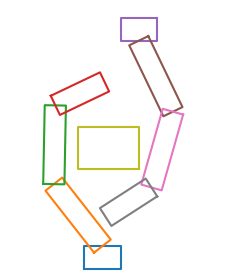
\includegraphics[width=\hsize]{fig/3-new-planner/rec_before_FC.png}
\subcaption{Before applying}\label{fig::planner::beforefc}
\end{minipage}\hfill
\begin{minipage}{0.33\hsize}
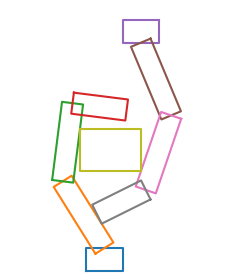
\includegraphics[width=\hsize]{fig/3-new-planner/rec_FC_left_right.png}
\subcaption{left$\rightarrow$right}\label{fig::planner::afterfclr}
\end{minipage}\hfill
\begin{minipage}{0.33\hsize}
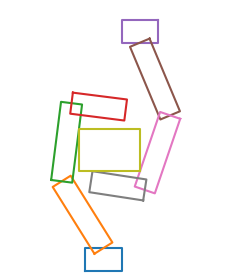
\includegraphics[width=\hsize]{fig/3-new-planner/rec_FC_right_left.png}
\subcaption{right$\rightarrow$left}\label{fig::planner::afterfcrl}
\end{minipage}
\caption{The result of applying hand closing algorithm}\label{fig::planner::fc}
\end{figure}

%%%%%%%%%%%%%%%%%%%%%%%%%%%%%%%%%%%%%%%%%%%%%%%%%%%%%%%%%%%%%%%%%%%%%%%%%%%%%%%%%%%%%%%%%%%%%%%%%%%%%%
%%%%%%%%%%%%%%%%%%%%%%%%%%%%%%%%%%%%%%%%%%%%%%%%%%%%%%%%%%%%%%%%%%%%%%%%%%%%%%%%%%%%%%%%%%%%%%%%%%%%%%
\section{逆探索アルゴリズム}\label{sec::planner::reverse}
\subsection{RRTを用いた逆探索アルゴリズム}
順探索アルゴリズムとは逆方向のアプローチを試みる.つまり,対象物が目標位置・姿勢で位置決めされた時のハンド姿勢$\bm{\theta_G}$を探索の開始点とし,マニピュレーションの初期状態$(t=0)$へと遡る方向へ探索することを考える.探索アルゴリズムにはRRTを用い,基本的には\ssecref{sec::sicm::planning}と同様で,ランダムサンプリング,ケージングに関する2条件の確認,ノードの追加を行っていき,探索終了条件を満たせば動作計画を終了する.この探索方法を逆探索アルゴリズムと呼ぶ.このアルゴリズムでは対象物を位置決めするハンド姿勢を探索開始点として与える必要がある.また,生成される動作の最終姿勢は,通常位置決め姿勢は複数あるが,与えた姿勢に限定される.その代わり,十分に位置決めされた姿勢を与えることができれば,位置決め精度の高いマニピュレーション動作を生成できることになる.


\subsubsection{ケージング成立条件とケージングマニピュレーション可能条件}\label{subsec::planner::revcm}
ケージング成立条件に関しては順探索アルゴリズムと同様である.ケージングマニピュレーション可能条件も条件自体は,\secref{sec::sicm::caging}と変わらない.ただ,時間が逆行した方向への探索であるため処理が異なる.処理は\figref{fig::planner::cm}のような3パターンに大別できる.ただし,実際の$\mathcal{C}_{\mathrm{free\_obj}}$領域は3次元であるが,\figref{fig::planner::cm}では簡単のため2次元としてモデル化している.\figref{fig::planner::cm1}は$C_{\mathrm{free\_obj}}(t)$に対してオーバーラップしている$C_{\mathrm{free\_obj}}(t-\Delta t)$が複数ある場合である.ここでケージングマニピュレーション可能条件は,時間$t-\Delta t$における物体の存在領域$\mathcal{C}_{\mathrm{free\_obj}}(t-\Delta t)$がどの領域に遷移したかを追跡するためにオーバーラップする$\mathcal{C}_{\mathrm{free\_obj}}(t)$の領域数を1つに絞るといったものであった.この観点で\figref{fig::planner::cm1}を見ると,各々の$C_{\mathrm{free\_obj}}(t-\Delta t)$から$C_{\mathrm{free\_obj}}(t)$の1領域のみとオーバーラップしており各々追跡可能なので,ケージングマニピュレーション可能条件を満たしているといえる.この判定は,逆探索アルゴリズムでは$C_{\mathrm{free\_obj}}$が複数個存在しうることを意味している.これを踏まえて,ケージングマニピュレーション可能条件をより正確に以下のように再定義する.
\begin{itemize}
\item $C_{\mathrm{free\_obj}}(t-\Delta t)$の各々の領域は$C_{\mathrm{free\_obj}}(t)$のある1つの領域のみとオーバーラップする
\end{itemize}

\figref{fig::planner::cm2}の状況も発生しうる.これは,$C_{\mathrm{free\_obj}}(t-\Delta t)$に対してオーバーラップしている$C_{\mathrm{free\_obj}}(t)$が複数あるので,ケージングマニピュレーション可能条件を満たしていない.\figref{fig::planner::cm3}では,そもそもオーバーラップがないので不成立である.以上の3つで全ての場合に対して判定することができる.

\begin{figure}[b]
\begin{minipage}{0.33\hsize}
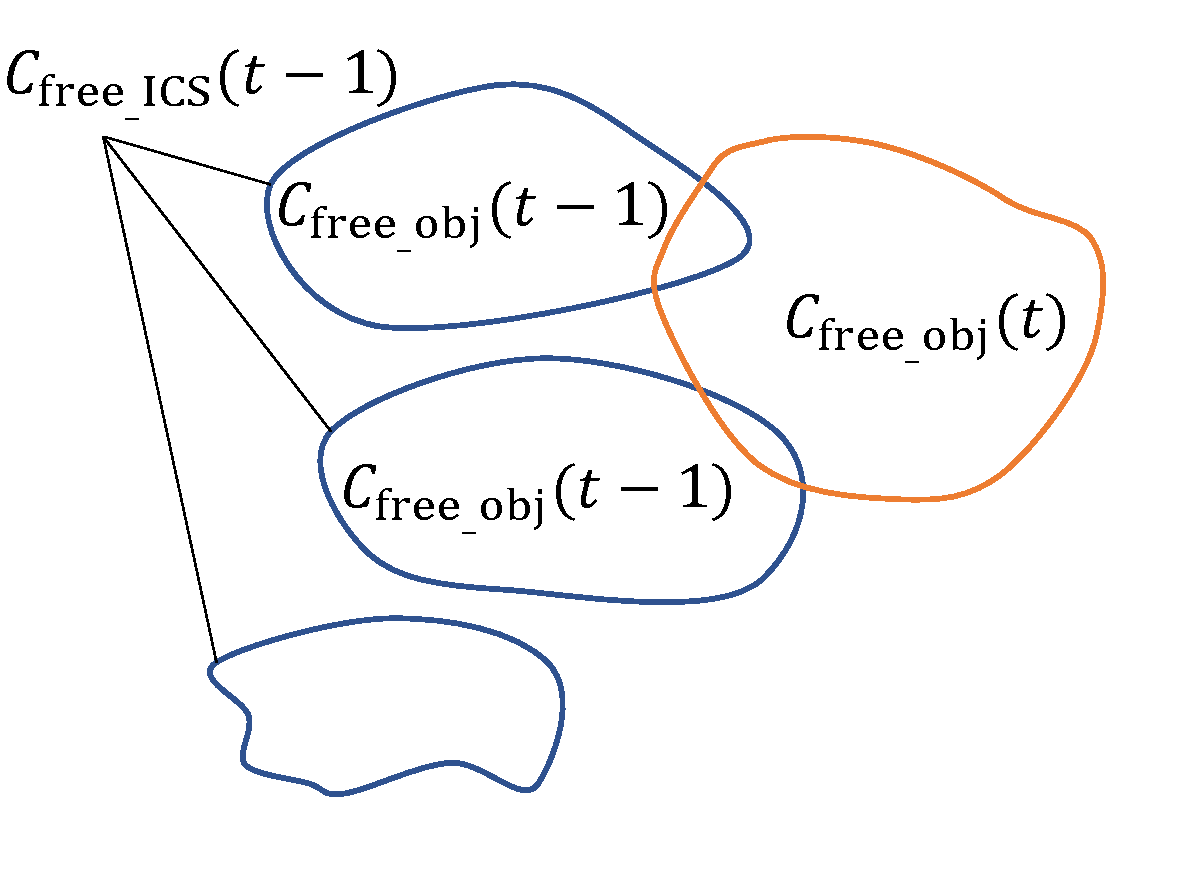
\includegraphics[width=\hsize]{fig/3-new-planner/rev_cagingmani_ver1.pdf}
\subcaption{}\label{fig::planner::cm1}
\end{minipage}\hfill
\begin{minipage}{0.33\hsize}
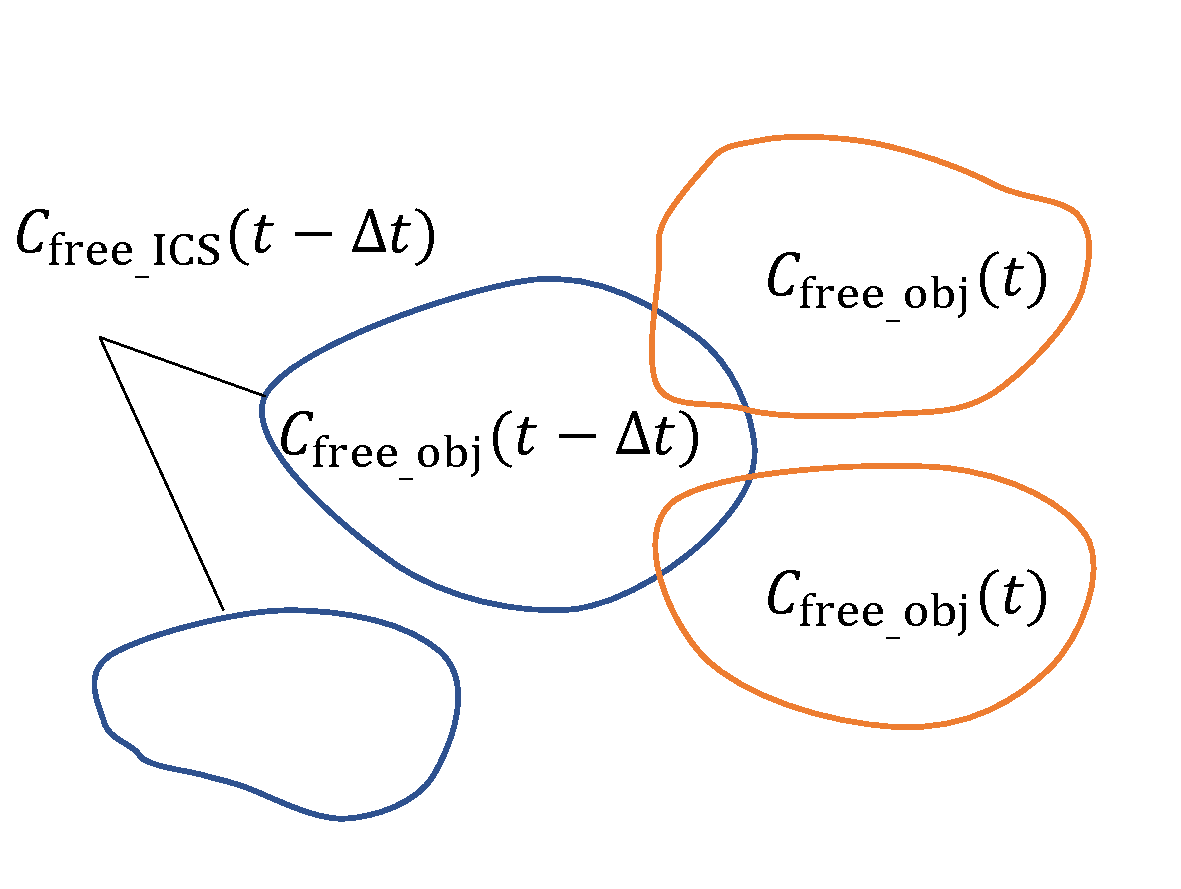
\includegraphics[width=\hsize]{fig/3-new-planner/rev_cagingmani_ver2.pdf}
\subcaption{}\label{fig::planner::cm2}
\end{minipage}\hfill
\begin{minipage}{0.33\hsize}
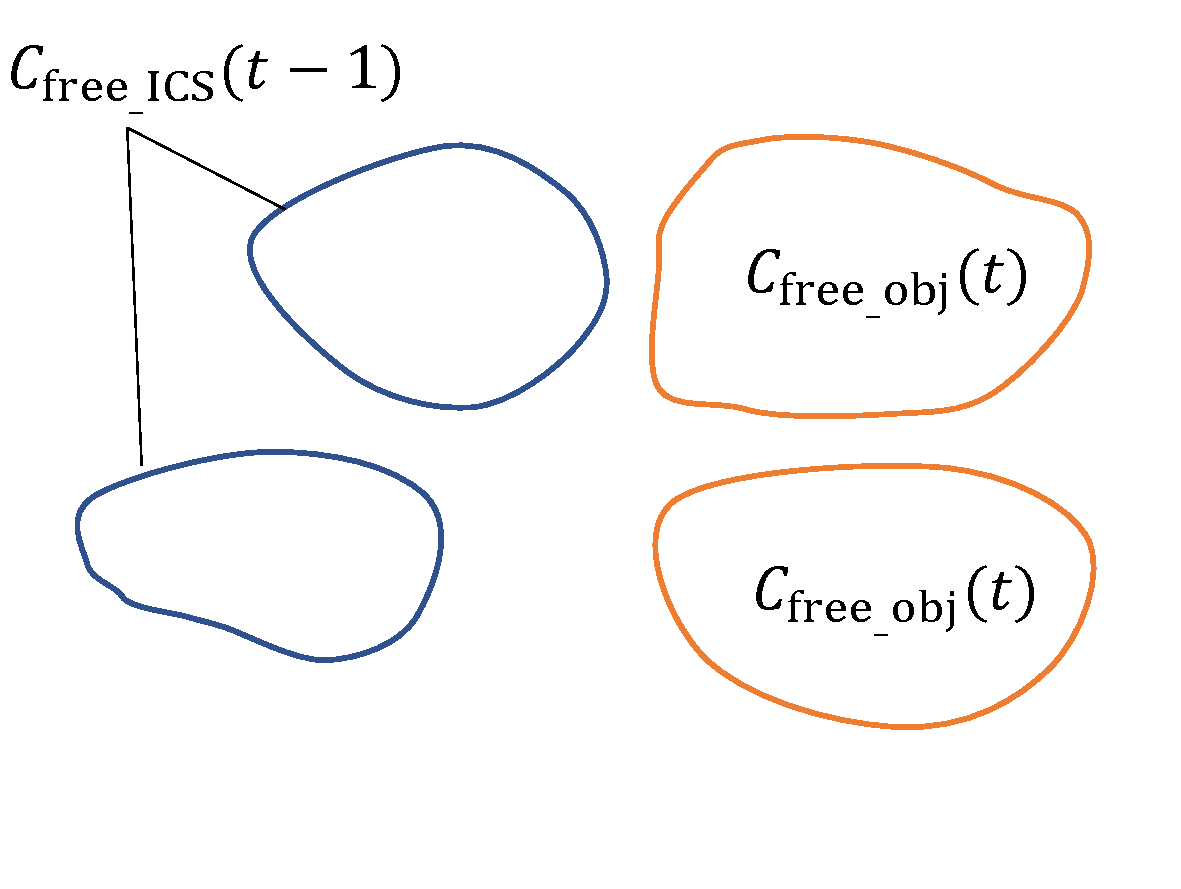
\includegraphics[width=\hsize]{fig/3-new-planner/rev_cagingmani_ver3.pdf}
\subcaption{}\label{fig::planner::cm3}
\end{minipage}
\caption{The patterns of the condition for caging manipulability for reverse exploring}
\label{fig::planner::cm}
\end{figure}

\subsubsection{逆探索アルゴリズムにおける$C_{\mathrm{free\_obj}}$の抽出}
逆探索アルゴリズムの$C_{\mathrm{free\_obj}}$抽出も\ssecref{subsec::planner::dfs}の考え方を基に実装する.まず,$t+\Delta t$における$C_{\mathrm{free\_obj}}(t+\Delta t)$の任意の点を起点として,深さ優先探索で$C_{\mathrm{free\_obj}}(t)$を抽出する.次に,$C_{\mathrm{free\_obj}}(t+\Delta t)$と$C_{\mathrm{free\_obj}}(t)$のオーバーラップを前項を基に考える.ここで,本実装では\ssecref{subsec::planner::dfs}の方法により,$C_{\mathrm{free\_obj}}$のみを抽出するようにしている.しかし通常,$C_{\mathrm{free\_obj}}$の周囲には別領域の$C_{\mathrm{free\_ICS}}$が存在している.したがって,$C_{\mathrm{free\_obj}}(t)$と$C_{\mathrm{free\_ICS}}(t+\Delta t)\, \ni C_{\mathrm{free\_obj}}(t+\Delta t)$のオーバーラップを考える必要がある.\par
そこで,$C_{\mathrm{free\_obj}}(t)$を起点として,再度$t+\Delta t$のハンド姿勢に対して\ssecref{subsec::planner::dfs}の方法で$C'_{\mathrm{free\_obj}}(t+\Delta t)$を抽出する.この$C'_{\mathrm{free\_obj}}(t+\Delta t)$の領域が0個もしくは複数個ある場合,ケージングマニピュレーション可能条件を満たさないので,$C_{\mathrm{free\_obj}}(t)$は妥当ではないと判定する.以上の処理を\algoref{algo::planner::revdfs}にまとめる.

\begin{algorithm}[tb]
\caption{Efficient extraction of $\mathcal{C}_{\mathrm{free\_obj}}$ for reverse search}
\label{algo::planner::revdfs}
\begin{algorithmic}[1]
\Require{current hand posture, $C_{\mathrm{free\_obj}}(t+\Delta t)$}
\Ensure{$C_{\mathrm{free\_obj}}(t)$}
\State{$C_{\mathrm{free\_obj}}(t) \gets \mathrm{empty}$}
%\State{Update the robot to `current hand posture'}
\ForEach{$c \in C_{\mathrm{free\_obj}}(t+\Delta t)$}
\State{$C_{\mathrm {free\_obj\_tmp}}=$ \Call{efficient\_extraction}{$c$, current hand posture}($\because$ \algoref{algo::planner::dfs})}
\ForEach{$c' \in C_{\mathrm{free\_obj\_tmp}}$}
\If{$c'$ is already existed in $C_{\mathrm{free\_obj}}(t)$}
\State{DELETE $c'$}
\State{\textbf{continue}}
\EndIf
\EndFor
\State{$C_{\mathrm{free\_obj}}(t) \xleftarrow{\mathrm{add}}  C_{\mathrm {free\_obj\_tmp}}$}
\EndFor
%\State{Update the robot to previous $(t+\Delta t)$ hand posture}
\ForEach{$c'' \in C_{\mathrm{free\_obj}}(t)$}
\State{$C_{\mathrm{free\_obj\_actual}}(t+\Delta t)=$ \Call{efficient\_extraction}{$c''$, previous hand posture}}
\IIf{The number of $C_{\mathrm{free\_obj\_actual}}(t+\Delta t) \neq 1$} DELETE  $c''$
\EndFor
%\State{Update the robot to `current hand posture'}
\State{\textbf{return} $C_{\mathrm{free\_obj}}(t)$}
\end{algorithmic}
\end{algorithm}

\subsubsection{探索終了条件}
逆探索であるため,探索の終了状態はマニピュレーションの初期状態に相当する.マニピュレーションの初期状態に求められることとしては,なるべく多様な対象物位置・姿勢を取り扱えるということが挙げられる.そこで,探索の終了条件を,物体が取りうる姿勢群を表す$\mathcal{C}_{\mathrm{free\_obj}}$の体積が閾値$\nu$以上になった時と定めた.
ここで,コンフィギュレーション空間の各離散点は,その点を中心とし,離散化幅$(\Delta x, \Delta y, \Delta \phi)$を3辺とするボクセルを占有すると考える.これを用いて体積は$(\mathcal{C}_{\mathrm{free\_obj}}を構成する離散点群の数)\times (ボクセル体積)$と定義している.\par
順探索アルゴリズムでは,ランダム探索なので対象物の目標位置・姿勢$P_G$から離れる方向へも探索が進むことがある.逆探索アルゴリズムでは探索の終了条件に座標の指定がなく,ただ$\mathcal{C}_{\mathrm{free\_obj}}$の領域を広げればよい.そのため,順探索のような無駄な探索方向が少なくっており,探索効率の改善が見込める.


\subsection{最適位置決め姿勢生成アルゴリズム}\label{subsec::planner::revoptimize}
逆探索アルゴリズムでは,対象物を目標位置・姿勢へ位置決めしたハンド姿勢を与える.これにより,人間が対象物を適切に位置決めできるハンド姿勢を与えることができれば,高い位置決め精度が保証された動作が生成される.一方,実際にハンドを動かして試行錯誤して位置決め姿勢を探し,ケージング成立条件を満たしているか確認するという作業は手間であるともいえる.人間が恣意的に与えるハンド姿勢は位置決めに最適ではない場合も多い.そこで,ハンドの位置決め姿勢を最適化計算によって算出する最適位置決め姿勢生成アルゴリズムを提案する.\par
最適化計算は,粒子群最適化法(Particle Swarm Optimization, PSO) \cite{kennedy1995}を用いて行う.PSOの概要について述べる.PSOは鳥や魚の群れ行動をモデル化した最適化手法である.探索空間に複数の粒子を配置し,粒子間で情報共有しながら最適な解を目指して粒子群を移動させていくアルゴリズムとなっている.粒子群の移動は位置と速度で制御する.各粒子の速度は慣性による方向,自身が移動してきた中で最良の位置(パーソナルベスト)へ向かう方向,粒子全体で最良の位置(グローバルベスト)へ向かう方向のベクトルで表される.式で表すと,粒子$i$の位置$x_i(t)$,速度$v_i(t)$は以下のようにあらわせる.

\begin{align}
&x_i(t) = x_i(t-1) + v_i(t-1) \label{eq::planner::posupdate} \\
&v_i(t) = wv_i(t-1) + c_1 r_1 (p^{\mathrm{best}}_i - x_i(t)) + c_2 r_2 (g^{\mathrm{best}}-x_i(t))\label{eq::planner::vecupdate}
\end{align}

ここで,$c_1$,$c_2$は[0, 1]の乱数,$w$,$r_1$,$r_2$は各ベクトルの重みを表し,$p^{\mathrm{best}}_i$は粒子$i$の最良解,$g^{\mathrm{best}}$は全粒子中の最良解を表す.
ハンドの最適姿勢を探すので,探索空間はハンドの関節角度からなる6自由度空間であり,位置,速度は6次元ベクトルで表される.具体的なアルゴリズムの流れは以下のようになっている.

\begin{enumerate}
\item 探索空間に全粒子をサンプリングする\label{alg::planner::pso::sampling}
\item \eqref{eq::planner::posupdate}に従って,各粒子の位置を更新する\label{alg::planner::pso::posupdate}
\item 更新された位置で評価を行う\label{alg::planner::pso::eval}
\item パーソナルベストとグローバルベストを更新する
\item \eqref{eq::planner::vecupdate}に従って,各粒子の速度を更新する
\item 指定した繰り返し回数内ならば,手順\ref{alg::planner::pso::posupdate}に戻る
\end{enumerate}

手順\ref{alg::planner::pso::eval}の評価値$E$は収束度$e$を用いて,以下の式で定義する.
\begin{gather}
\left\{
\begin{aligned}
&E=e & &(ケージング2条件成立)\\
&E=D_{\mathrm{far}} & &(\mathrm{otherwise})
\end{aligned}
\right .
\end{gather}
ケージング2条件を満たさないような妥当でない姿勢の時の評価値は悪くなるようにしたい.そこで,$D_{\mathrm{far}}$には通常収束度$e$が取りうる値より一回り大きい値を設定する.
また,手順\ref{alg::planner::pso::sampling}において,2つの用途を想定し2パターンのサンプリングを実装した.一つ目が,最適化計算のみによって最適位置決め姿勢を得たい場合である.この場合は,ハンドの関節角度$\theta_i$の可動範囲$-90 \leq \theta_i \leq 90 \mathrm{[deg]}$に対してランダムにばらまく.しかし,探索領域が広いため,収束までの繰り返し計算回数が多くなる.また,局所解に収束する場合も多く見られた.二つ目が,人間が簡易的な位置決め姿勢を与えたり,順探索アルゴリズムで生成された動作の最終姿勢を参照したりなどで,ある程度の位置決め姿勢が与えられる場合である.この場合は,与えられた関節角度から$\pm 10 \mathrm{[deg]}$の範囲内にばらまく.これにより,前者よりは少ない繰り返し回数で最適解に収束できる.\par

三角形物体に対して,以下のようにパラメータ設定し,最適化を行った.手順\ref{alg::planner::pso::sampling}には,後者の簡易的な位置決め姿勢を与え,その周囲$\pm 10 \mathrm{[deg]}$に粒子群をばらまく方法を取った.
\begin{gather}
\left\{
\notag
\begin{aligned}
&簡易的な位置決め姿勢:[50, -60, 5, 10, -10, -80]\mathrm{[deg]}\\
&対象物の目標位置・姿勢:(x, y, \phi) = (\mathrm{any}, 180, 0)\\
&w=0.5, \: r_1=0.7, \: r_2 = 0.5\\
&D_{\mathrm{far}}=1000\\
&粒子群数:50\\
&繰り返し回数:100
\end{aligned}
\right .
\end{gather}

結果,位置決め姿勢:$[47.3, -63.8, 3.17, 5.7, -8.5, -77.3]\mathrm{[deg]}$が得られ,評価値$E=0$で,収束度も$e=0$であった.これにより,本最適化手法によって逆探索アルゴリズムの入力に必要な位置決め姿勢を生成できることが確認された.

\subsection{探索結果}\label{subsec::planner::revresult}
\begin{figure}[b]
\centering
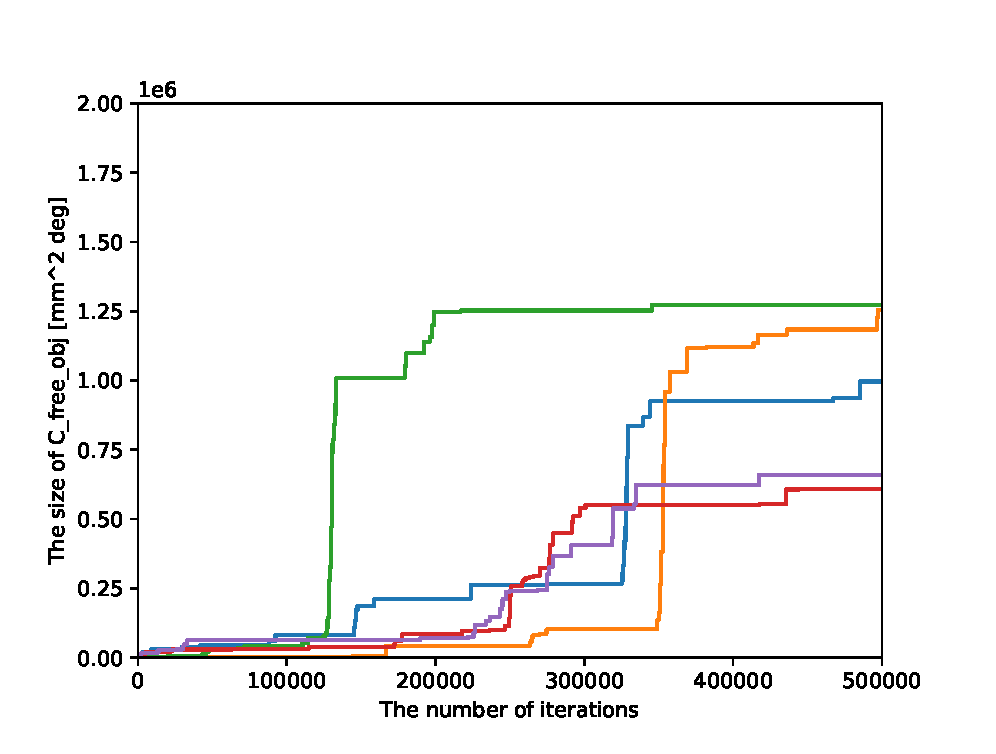
\includegraphics[width=0.7\hsize]{fig/3-new-planner/transition_vol.eps}
\caption{The transition of the size of $\mathcal{C}_{\mathrm{free\_obj}}$}\label{fig::planner::revrrtres}
\end{figure}
順探索アルゴリズムと計算時間の比較を行いたいが,問題設定が異なるため直接比較することはできない.そこで,繰り返し回数に対する$\mathcal{C}_{\mathrm{free\_obj}}$の体積の推移を紹介し,その結果をもとに簡易的に順探索アルゴリズムと比較する.以下のようなタスクを設定し,5回探索を行ったときの結果を\figref{fig::planner::revrrtres}に示す.なお,本来は$\mathcal{C}_{\mathrm{free\_obj}}$の体積が閾値$\nu$を超えたときに探索が終了するが,今回は500000回の繰り返し計算を行うと終了するように設定した.ハンド最終姿勢には,前項で算出したハンド姿勢を用いる.

\begin{gather}
\notag
\left\{
\begin{aligned}
&ハンド最終姿勢(位置決め姿勢):[\theta_1, \theta_2, \theta_3, \theta_4, \theta_5, \theta_6,]\\
&                  = [47.3, -63.8, 3.17, 5.7, -8.5, -77.3]\mathrm{[deg]}\\
&探索終了閾値:繰り返し計算数が500000回に到達\\
&対象物:三角形物体
\end{aligned}
\right .
\end{gather}

順探索アルゴリズムで三角形物体の動作計画を行う時,入力するハンド初期姿勢$C_{\mathrm{free\_obj}}$の点群数は500程度であることが多い.そこで,\figref{fig::planner::revrrtres}において点群数500にボクセル体積$500 \mathrm{[mm^2 \cdot deg]}$をかけた$250000 \mathrm{[mm^2 \cdot deg]}$に到達した時の繰り返し計算回数に注目することで簡易的に比較できる.5回の平均を取ると,繰り返し回数が約245000回の時に到達している.逆探索アルゴリズムでは,繰り返し計算1回にかかる時間は約1[ms]なので,約245[s]と算出される.
順探索アルゴリズムの結果\tabref{tab::planner::rasterdfs}と計算時間を比較すると,平均値は逆探索アルゴリズムの方が約$31\%$短くなった.


%%%%%%%%%%%%%%%%%%%%%%%%%%%%%%%%%%%%%%%%%%%%%%%%%%%%%%%%%%%%%%%%%%%%%%%%%%%%%%%%%%%%%%%%%%%%%%%%%%%%%%
%%%%%%%%%%%%%%%%%%%%%%%%%%%%%%%%%%%%%%%%%%%%%%%%%%%%%%%%%%%%%%%%%%%%%%%%%%%%%%%%%%%%%%%%%%%%%%%%%%%%%%
\section{両側探索アルゴリズム}\label{sec::planner::connect}
更なる計算速度の向上を目指して,順探索アルゴリズムと逆探索アルゴリズムを組み合わせた両探索アルゴリズムを提案する.
\subsection{RRT-Connectを用いた両側探索アルゴリズム}
RRT-Connect \cite{kuffner2000}を用いて両側探索アルゴリズムを構築する.これは,順探索アルゴリズムにおける探索初期状態$\bm {\theta}_S$と逆探索アルゴリズムにおける探索初期状態$\bm {\theta}_G$から交互に枝を伸ばしていき,これらの枝が連結した時,その連結経路を解として探索を終了するアルゴリズムである.なお,本アルゴリズムでは順探索アルゴリズム,逆探索アルゴリズムの探索終了条件も残しており,合計3つの探索終了条件の内,いずれかを満たせば終了するようになっている.具体的なアルゴリズムは以下のようになっている(\figref{fig::planner::rrtconnect}).
\begin{enumerate}
\item 順探索におけるハンドの初期ノード(姿勢)$\bm{q}_{\mathrm {init}}$と逆探索におけるハンドの初期ノード$\bm{q}_{\mathrm {goal}}$を設定する.以降,$\bm{q}_{\mathrm {init}}$を起点としたグラフを$T_{\mathrm {forward}}$,$\bm{q}_{\mathrm {goal}}$を起点としたグラフを$T_{\mathrm {reverse}}$とする
\item ハンドの任意のノード$\bm{q}_{\mathrm {sample}}$をサンプリングし,$T_{\mathrm {forward}}$の内,$\bm{q}_{\mathrm{sample}}$から最も近いノード$\bm{q}_{\mathrm{nearest}}$を見つける\label{algo::planner::sampling}
\item $\bm{q}_{\mathrm{nearest}}$から$\bm{q}_{\mathrm{sample}}$の方向へ長さ$\Delta l$の枝を伸ばし,そのノードを$\bm{q}_{\mathrm{new}}$とする \label{algo::planner::qnew}
\item $\bm{q}_{\mathrm{new}}$において環境とハンドまたはハンド同士の干渉,ケージングに関する2条件を判定し,妥当でなければ手順\ref{algo::planner::sampling}に戻る
\item $\bm{q}_{\mathrm{new}}$と一番近いノード$\bm{q}_{\mathrm{opposite\_near}}$を$T_{\mathrm {reverse}}$から探索する\label{algo::planner::biasbegin}
\item $\bm{q}_{\mathrm{opposite\_near}}$から$\bm{q}_{\mathrm{new}}$に向けて長さ$\Delta l$の枝を伸ばし,$\bm{q}_{\mathrm{opposite\_new}}$とする\label{algo::planner::proceed}
\item $\bm{q}_{\mathrm{opposite\_new}}$において環境とハンドまたはハンド同士の干渉,ケージングに関する2条件を判定する
\item $\bm{q}_{\mathrm{opposite\_new}}$が妥当かつ探索終了条件を満たさない場合,$\bm{q}_{\mathrm{opposite\_new}}$を$\bm{q}_{\mathrm{opposite\_near}}$とし,手順\ref{algo::planner::proceed}に戻る\label{algo::planner::biasend}
\item $\bm{q}_{\mathrm{opposite\_new}}$が妥当でない場合,役割を入れ替えて(詳細は後述する),手順\ref{algo::planner::sampling}に戻る \label{algo::planner::change}
\item $\bm{q}_{\mathrm{opposite\_new}}$が探索終了条件を満たせば終了\label{algo::planner::goalcond}
\end{enumerate}

手順\ref{algo::planner::change}の役割を入れ替えるという部分は具体的には以下のことを行う.
\begin{itemize}
\item 手順\ref{algo::planner::sampling}の$T_{\mathrm {forward}}$と$T_{\mathrm {reverse}}$を入れ替える
\item 手順\ref{algo::planner::biasbegin}の$T_{\mathrm {reverse}}$と$T_{\mathrm {forward}}$を入れ替える
\end{itemize}

\begin{figure}[b]
\centering
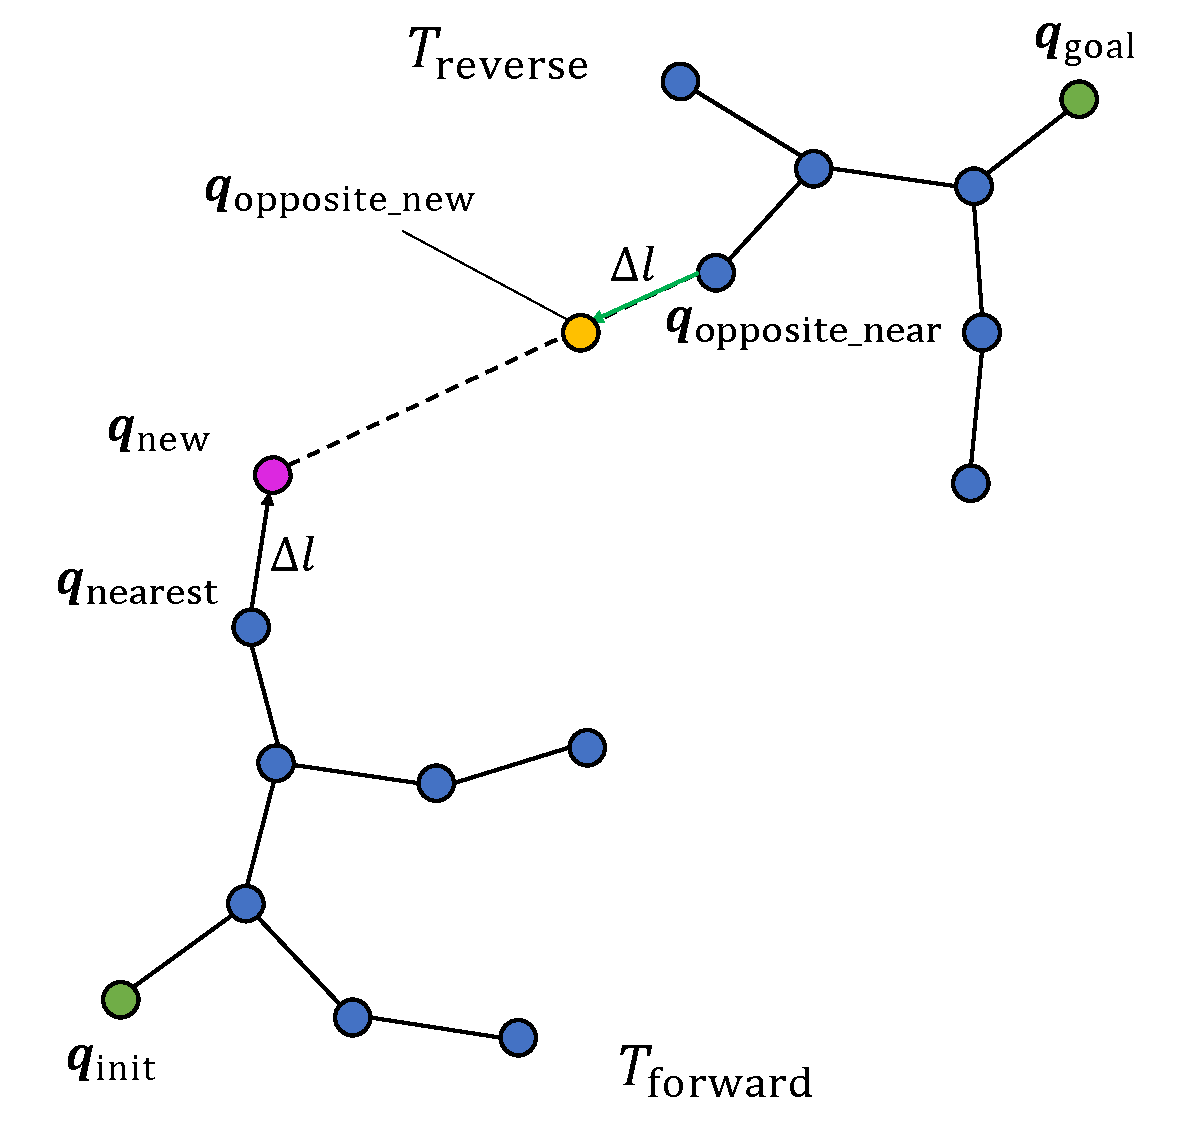
\includegraphics[width=0.6\hsize]{fig/3-new-planner/RRTConnect.pdf}
\caption{Procedure of RRT-Connect}
\label{fig::planner::rrtconnect}
\end{figure}

本アルゴリズムの特徴は三つある.一つ目は,探索終了条件を3つ設定していることである.それぞれ,(a)$T_{\mathrm {forward}}$が順探索アルゴリズムの探索終了条件を満たす,(b)$T_{\mathrm {reverse}}$が逆探索アルゴリズムの探索終了条件を満たす,(c)$T_{\mathrm {forward}}$と$T_{\mathrm {reverse}}$が繋がり,結合点間のケージング2条件も満たす,の3つとなっている.なお,経路生成後,必要に応じて,\ssecref{subsec::planner::formclosure}の位置決め精度向上アルゴリズムを適用する.3つの探索終了条件の内,いずれかを満たせばよいため,順探索アルゴリズム,逆探索アルゴリズムと比べて条件は緩くなっていると言える.二つ目は,手順\ref{algo::planner::biasbegin}から\ref{algo::planner::biasend}にかけて非常に強いバイアスがかかるという点である.スタートからゴール方向へ,ゴールからスタート方向へ進めるだけ進めるというバイアスがかかっているため,順探索アルゴリズムや逆探索アルゴリズムのようなランダムサンプリングに比べて効率的な探索になっている.三つ目は,経路が比較的滑らかなことである.順探索アルゴリズム,逆探索アルゴリズムではランダムに枝を伸ばしていくため,凹凸の多い経路が生成される.このような経路では,マニピュレーションにかかる時間が増加したり,関節部にかかる負荷が大きくなったりといったことが考えられる.一方,本探索手法では手順\ref{algo::planner::proceed}において一直線に枝を伸ばすような探索が行われるので,順探索アルゴリズム,逆探索アルゴリズムに比べて滑らかな経路が生成される.

\subsection{計算時間の比較}
両側探索アルゴリズムは,順探索アルゴリズムにマニピュレーション終了状態のハンド姿勢を,逆探索アルゴリズムにマニピュレーション初期状態のハンド姿勢を追加で与え,これら追加情報を活用して探索を効率化するアルゴリズムである.この追加情報によって順探索アルゴリズム,逆探索アルゴリズムそれぞれからどの程度,計算速度が速くなるかを検証する.\par
L字形物体に対して,タスクを以下のように設定した.20回分の計算時間を計測し,その結果を\tabref{tab::planner::LFB},\figref{fig::planner::LFB}に示す.
\begin{gather}
\notag
\left\{
\begin{aligned}
&ハンド初期姿勢:[\theta_1, \theta_2, \theta_3, \theta_4, \theta_5, \theta_6,] = [40, -50, -30, 40, -50, -30]\mathrm{[deg]}\\
&ハンド最終姿勢:[\theta_1, \theta_2, \theta_3, \theta_4, \theta_5, \theta_6,] = [12, -15, -25, 5, 30, -90]\mathrm{[deg]}\\
&対象物:\mathrm{L}字形物体\\
&対象物の目標位置・姿勢:[x_{\mathrm {goal}}, y_{\mathrm {goal}}, \phi_{\mathrm {goal}}] = [{\mathrm {any}}, 200 \mathrm{[mm]}, 0 \mathrm{[deg]}]\\
&順探索の終了閾値:\varepsilon = 50\\
&逆探索の終了閾値:\nu = 500000 \mathrm{[mm^2 \cdot deg]} = 0.5 \mathrm{[m^2 \cdot deg]}
\end{aligned}
\right .
\end{gather}

\begin{table}[t]
    \centering
    \caption{Comparison of calculation time between forward search, reverse search and bidirectional search for L-Shape object}
    \label{tab::planner::LFB}
    \begin{tabular}{c|r r r}
        ~ & 
        \begin{tabular}{c}
        Forward search \\ $\mathrm{\, [s]}$
        \end{tabular}
        &
         \begin{tabular}{c}
        Reverse search \\ $\mathrm{\, [s]}$
        \end{tabular}
         & 
          \begin{tabular}{c}
        Bidirectional search \\ $\mathrm{\, [s]}$
        \end{tabular}
         \\ \hline
        1 & 614.1 & 430.7& 19.5 \\ 
        2 & 569.2 & 88.6& 85.4 \\ 
        3 & 1097.1 & 104.4 & 11.0 \\
        4 & 117.3 & 135.0 & 19.2 \\
        5 & 285.8 & 221.1 & 63.5 \\
        6 & 176.9 & 98.0 & 26.1 \\
        7 & 457.0 & 314.4 & 101.1 \\
        8 & 650.1 & 434.3 & 12.3 \\
        9 & 1219.7 & 56.8 & 48.1 \\
        10 & 2341.8 & 1222.9 & 33.3 \\
        11 & 113.7 & 609.1 & 12.2 \\
        12 & 2048.0 & 264.6 & 14.9 \\
        13 & 939.6 & 741.9 & 52.0 \\
        14 & 41.9 & 69.8 & 60.9 \\
        15 & 848.5 & 1000.4 & 20.6 \\ 
        16 & 2760.0 & 777.9 & 22.7 \\ 
        17 & 2410.0 & 1134.0 & 8.2 \\
        18 & 375.6 & 170.3 & 155.4 \\ 
        19 & 229.4 & 113.5 & 19.2 \\ 
        20 & 225.4 & 390.67 & 81.5 \\ \hline
        Average & 877.4  & 418.9 & 43.4 \\ \hline
        SD & 850.1 & 372.7 & 38.4 \\ 
    \end{tabular}
\end{table}
\begin{figure}[hb]
\centering
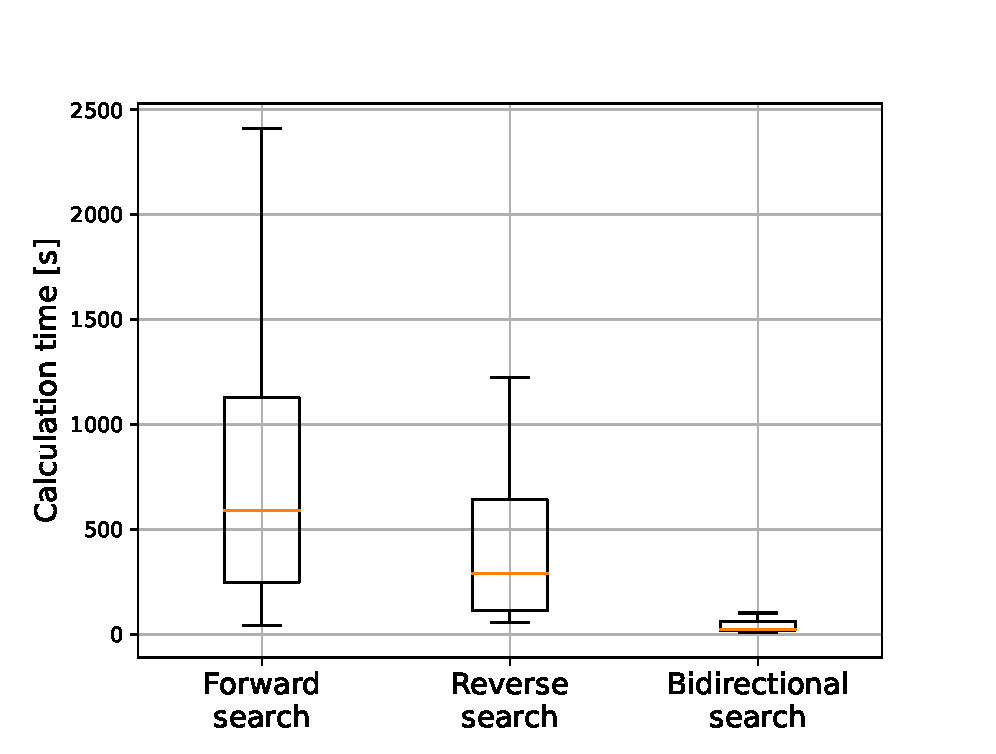
\includegraphics[width=0.5\hsize]{fig/3-new-planner/3_4_1.eps}
\caption{The box plot comparing calculation time between forward search, reverse search and bidirectional search for L-Shape object}
\label{fig::planner::LFB}
\end{figure}


\clearpage
\subsubsection*{順探索アルゴリズムと両側探索アルゴリズムの比較}
まず,2つのデータが等分散か否かを$F$検定により判断する.有意水準$5\%$とし,両側検定を行う.
\begin{gather}
\left\{
\notag
\begin{aligned}
&帰無仮説& &H_0:\sigma_1^2 = \sigma_2^2\\
&対立仮説& &H_1:\sigma_1^2 \neq \sigma_2^2\\
&検定統計量& &T = \dfrac{s_1^2}{s_2^2} = 489.6\\
&棄却域& &F(f_1, f_2; \alpha/2)=F(19, 19; 0.025) = 2.53\\
\end{aligned}
\right .
\end{gather}
$T=489.6 > 2.53$なので,$H_0$は棄却され,2つのデータは等分散ではないといえる.\par
2つのデータは非等分散なので,ウェルチの$t$検定により両側探索アルゴリズムの平均計算時間が順探索アルゴリズムに比べて有意に短いことを示す.
有意水準を$5\%$とし,片側検定を行う.
\begin{gather}
\left\{
\notag
\begin{aligned}
&帰無仮説& &H_0:\mu_1 = \mu_2\\
&対立仮説& &H_1:\mu_1 \neq \mu_2\\
&検定統計量& &T = \dfrac{\overline{x}_{1}-\overline{x}_{2}}{\sqrt{\dfrac{s_1^{2}}{n_{1}}+\dfrac{s_2^{2}}{n_{2}}}} = 4.38\\
&自由度& &f=\dfrac{1}{\dfrac{C^2}{n_1-1}+\dfrac{(1-C)^2}{n_2-1}}=19.1\simeq 19 & \because C=\dfrac{\dfrac{s_1^2}{n_1}}{\dfrac{s_1^2}{n_1}+\dfrac{s_2^2}{n_2}}\\
&棄却域& &t(f, \alpha/2) = t(19, 0.05) = 2.093
\end{aligned}
\right .
\end{gather}
$T=4.38 > 1.729$なので,$H_0$は棄却され,両側探索アルゴリズムの計算時間は順探索アルゴリズムに比べて有意に短いことが示された.


\subsubsection*{逆探索アルゴリズムと両側探索アルゴリズムの比較}
前項同様,まず2つのデータが等分散か否かを$F$検定により判断する.有意水準$5\%$とし,両側検定を行う.
\begin{gather}
\left\{
\notag
\begin{aligned}
&帰無仮説& &H_0:\sigma_1^2 = \sigma_2^2\\
&対立仮説& &H_1:\sigma_1^2 \neq \sigma_2^2\\
&検定統計量& &T = \dfrac{s_1^2}{s_2^2} = 94.1\\
&棄却域& &F(f_1, f_2; \alpha/2)=F(19, 19; 0.025) = 2.53\\
\end{aligned}
\right .
\end{gather}
$T=94.1 > 2.53$なので,$H_0$は棄却され,2つのデータは等分散ではないといえる.\par
2つのデータは非等分散なので,ウェルチの$t$検定により両側探索アルゴリズムの平均計算時間が逆探索アルゴリズムに比べて有意に短いことを示す.
有意水準を$5\%$とし,片側検定を行う.
\begin{gather}
\left\{
\notag
\begin{aligned}
&帰無仮説& &H_0:\mu_1 = \mu_2\\
&対立仮説& &H_1:\mu_1 \neq \mu_2\\
&検定統計量& &T = \dfrac{\overline{x}_{1}-\overline{x}_{2}}{\sqrt{\dfrac{s_1^{2}}{n_{1}}+\dfrac{s_2^{2}}{n_{2}}}} = 4.48\\
&自由度& &f=\dfrac{1}{\dfrac{C^2}{n_1-1}+\dfrac{(1-C)^2}{n_2-1}}=19.4 \simeq 19 & \because C=\dfrac{\dfrac{s_1^2}{n_1}}{\dfrac{s_1^2}{n_1}+\dfrac{s_2^2}{n_2}}\\
&棄却域& &t(f, \alpha/2) = t(19, 0.05) = 2.093
\end{aligned}
\right .
\end{gather}
$T=4.48 > 1.729$なので,$H_0$は棄却され,両側探索アルゴリズムの計算時間は逆探索アルゴリズムに比べて有意に短いことが示された.

%\begin{gather}
%\notag
%\left\{
%\begin{aligned}
%&ハンド初期姿勢:[\theta_1, \theta_2, \theta_3, \theta_4, \theta_5, \theta_6,] = [40, -50, -30, 40, -50, -30]\mathrm{[deg]}\\
%&ハンド最終姿勢:[\theta_1, \theta_2, \theta_3, \theta_4, \theta_5, \theta_6,] = []\mathrm{[deg]}\\
%&対象物:\mathrm{T}字形物体\\
%&対象物の目標位置・姿勢:[x_{\mathrm {goal}}, y_{\mathrm {goal}}, \phi_{\mathrm {goal}}] = [{\mathrm {any}}, 200 \mathrm{[mm]}, 0 \mathrm{[deg]}]\\
%&順探索の終了閾値:\varepsilon = 50\\
%&逆探索の終了閾値:\nu = 1000
%\end{aligned}
%\right .
%\end{gather}
%20回動作計画を行い,計算時間を計測した.結果は\tabref{tab::planner::TRB}のようになった.
%\begin{table}[bt]
%    \centering
%    \caption{Comparison of calculation time between reverse search and bidirectional search}
%    \label{tab::planner::TRB}
%    \begin{tabular}{|c|c|c|}
%    \hline
%        ~ & Reverse search & Bidirectional search \\ \hline
%        1 & 44.2 [s] & 2.5 [s] \\ \hline
%        2 & 3.3 & 5.5 \\ \hline
%        3 & 3.6 & 3.6 \\ \hline
%        4 & 14.1 & 4.4 \\ \hline
%        5 & 302.6 & 3.1 \\ \hline
%        6 & 119.6 & 4.1 \\ \hline
%        7 & 16.3 & 2.5 \\ \hline
%        8 & 22.2 & 2.1 \\ \hline
%        9 & 9.07 & 3.9 \\ \hline
%        10 & 11.1 & 3.2 \\ \hline
%        11 & 82.6 & 3.0 \\ \hline
%        12 & 59.2 & 1.8 \\ \hline
%        13 & 33.5 & 2.4 \\ \hline
%        14 & 43.2 & 2.2 \\ \hline
%        15 & 265.3 & 2.7 \\ \hline
%        16 & 223.1 & 2.8 \\ \hline
%        17 & 107.7 & 3.5 \\ \hline
%        18 & 3.6 & 3.2 \\ \hline
%        19 & 48.4 & 2.8 \\ \hline
%        20 & 33.3 & 2.4 \\ \hline
%        Average & 72.3 [s]  & 3.1 [s] \\ \hline
%        SD & 89.7 [s] & 0.9 [s] \\ \hline
%    \end{tabular}
%\end{table}
%2つのデータが等分散か否かを$F$検定により判断する.有意水準$5\%$とし,両側検定を行う.
%\begin{gather}
%\left\{
%\notag
%\begin{aligned}
%&帰無仮説& &H_0:\sigma_1^2 = \sigma_2^2\\
%&対立仮説& &H_1:\sigma_1^2 \neq \sigma_2^2\\
%&検定統計量& &T = \dfrac{s_1^2}{s_2^2} = 489.6\\
%&棄却域& &F(f_1, f_2; \alpha/2)=F(19, 19; 0.025) = 2.53\\
%\end{aligned}
%\right .
%\end{gather}
%$T=489.6 > 2.53$なので,$H_0$は棄却され,2つのデータは等分散ではないといえる.\par
%2つのデータは非等分散なので,ウェルチの$t$検定により両側探索アルゴリズムの平均計算時間が順探索アルゴリズムに比べて有意に短いことを示す.
%有意水準を$5\%$とし,両側探索を行う.
%\begin{gather}
%\left\{
%\notag
%\begin{aligned}
%&帰無仮説& &H_0:\mu_1 = \mu_2\\
%&対立仮説& &H_1:\mu_1 \neq \mu_2\\
%&検定統計量& &T = \dfrac{\overline{x}_{1}-\overline{x}_{2}}{\sqrt{\dfrac{s_1^{2}}{n_{1}}+\dfrac{s_2^{2}}{n_{2}}}} = 4.38\\
%&自由度& &f=\dfrac{1}{\dfrac{C^2}{n_1-1}+\dfrac{(1-C)^2}{n_2-1}}=19.1\simeq 19 & \because C=\dfrac{\dfrac{s_1^2}{n_1}}{\dfrac{s_1^2}{n_1}+\dfrac{s_2^2}{n_2}}\\
%&棄却域& &t(f, \alpha/2) = t(19, 0.025) = 2.093
%\end{aligned}
%\right .
%\end{gather}
%$T=4.38 > 2.093$なので,$H_0$は棄却され,両側探索アルゴリズムの計算時間は順探索アルゴリズムに比べて有意に短いことが示された.

%%%%%%%%%%%%%%%%%%%%%%%%%%%%%%%%%%%%%%%%%%%%%%%%%%%%%%%%%%%%%%%%%%%%%%%%%%%%%%%%%%%%%%%%%%%%%%%%%%%%%%
\section{各アルゴリズムの利点・欠点}
以上,順探索アルゴリズム,逆探索アルゴリズム,両側探索アルゴリズムの3つを紹介した.いずれのアルゴリズムの利点と欠点があり,ニーズに応じてこれらのアルゴリズムを使い分けることが望ましい.本節では,各アルゴリズムの利点・欠点とどのような場合にどのアルゴリズムが便利かについて述べる.\par

まず,順探索アルゴリズムについてである.このアルゴリズムの利点は,対象物の目標位置・姿勢$P_{G} (x_{G}, y_{G}, \phi_{G})$の入力から,そこに位置決めできるハンド姿勢が生成される点にある.対象物形状が複雑になると,目標位置・姿勢$P_G$へ位置決めできるハンド姿勢を手動で見つけるのは困難な場合がある.このような場合,順探索アルゴリズムでは収束度$e$という位置決めの評価指標を用いて位置決めに適切なハンド姿勢を探索でき,有用である.欠点は,前述の通り計算時間が遅いことである.逆探索アルゴリズムとは厳密に比較できないが概ね遅くなっており,両側探索アルゴリズムと比べると明らかに遅かった.また,初期姿勢を与えるのが困難,手間であるという点も挙げられる.任意に初期姿勢を与えた場合,その姿勢がケージングを満たしているか,様々な対象物位置・姿勢を取り扱えるかなどを確かめる必要がある.加えて,与えた初期姿勢によっては目標位置・姿勢までの経路が存在しない,またはそのような経路を見つけるのが困難な場合があり,慎重にハンド初期姿勢を与える必要がある.\par

次に,逆探索アルゴリズムについてである.このアルゴリズムの利点は,指定が難しいハンド初期姿勢を自動で生成できる点にある.ハンドの初期姿勢は上述のような条件を満たす必要があり,ユーザが任意に与えるのは困難,手間である.そのため,「対象物の取りうる位置・姿勢群数が閾値以上」という条件を与えて探索し,これを満たし次第,ハンドの初期姿勢を得ることができる逆探索アルゴリズムは利便性が高い.また,対象物を位置決めできるハンド姿勢を与えるという点について,上述の通りハンドの位置決め姿勢を与えるのは困難な場合もあるが,対象物形状がシンプルな場合,人間の方が即座に適した姿勢を見つけることができる場合がある.また,最適位置決め姿勢生成アルゴリズムを使う手もある.適切に位置決めされたハンド姿勢を与えることができれば,ハンドは最適な姿勢へ推移していくことになり,かつ指定が難しい初期姿勢も計算で自動的に算出してくれるため非常に有用である.欠点としては,順探索アルゴリズムと同様,与えた位置決め姿勢から初期姿勢までの経路が存在しない,またはそのような経路を見つけるのが困難な場合があるということが挙げられる.\par


最後に,両側探索アルゴリズムについてである.利点は計算時間が最も短い点である.\secref{sec::planner::connect}の通り,順探索アルゴリズム,逆探索アルゴリズムに比べて計算時間が有意に短いことが示されており,有用性が高くなっている.二つ目の利点は,経路生成の成功率が高い点である.順探索アルゴリズム,逆探索アルゴリズムの共通の欠点として,与える情報によっては経路が存在しない,またはそのような経路を見つけるのが困難な場合があることを述べた.これに対して,両側探索アルゴリズムでは3つの探索終了条件を設定しているため,いずれかの入力情報が不適切でも経路が生成される可能性が残っている.例えば与えたマニピュレーション初期姿勢が適切ではなく,目標位置・姿勢までの経路が存在しない場合,つまり順探索方向に経路が存在しない場合でも,逆探索方向で経路が生成されうる.また,順探索アルゴリズムや逆探索アルゴリズムのようなランダム探索において,経路を見つけるのが非常に困難な場合でも,両側探索アルゴリズムの強力なバイアスによって経路を見つけやすくなっていると考えられる.欠点としては,与える情報がマニピュレーション初期姿勢,対象物位置決め姿勢など,上記アルゴリズム2つに比べて多いことが挙げられる.対象物が複雑形状で,与える姿勢の見当がつかない場合,両側探索アルゴリズムを適用するのは困難になる.\par

これらを踏まえて,どのようなシチュエーションにどのアルゴリズムが適しているかを考える.
まず,任意対象物を本システムでマニピュレーションするのが初めてなどの理由で,どのようなハンド位置決め姿勢が適しているか等の知見がなく,また人間が与えるのも困難な場合,順探索アルゴリズムを用いるのが望ましい.最初は,なるべく多様な位置・姿勢群を扱えるというようなことは考えず,ひとまずケージングを満たしている初期姿勢を与える.これに対して,順探索アルゴリズムで動作計画を行うことで,ハンド位置決め姿勢を得ることができる.また,このようなシチュエーションには最適位置決め姿勢生成アルゴリズムを用いる手もある.位置決め姿勢のみを得たいのか,経路も生成したいのかによって使い分けることが望ましい.\par
次に,任意対象物を位置決めできる姿勢が容易に準備できる,または上記のタスクによってハンド位置決め姿勢を得ている前提で,なるべく多様な位置・姿勢群を扱えるようなマニピュレーション初期姿勢を探索したい場合,逆探索アルゴリズムを用いるのが望ましい.探索終了条件に関して,\secref{sec::planner::reverse}のように$\mathcal{C}_{\mathrm{free\_obj}}$の体積が閾値$\nu$以上になった時というような設定でも良いが,\ssecref{subsec::planner::revresult}のように繰り返し回数(時間)で与えることもできる.これは,例えば限られた短い時間で可能な限り扱える位置・姿勢群を増やすといった用途に役立つ設定となっている.このように探索終了条件においてもニーズに応じた設定が可能である.\par
最後に,任意対象物をマニピュレーションするにあたって,ある程度の知見があり動作計画にかかる時間を重視する場合,両側探索アルゴリズムが適している.他には,経路を見つけやすいという観点から順探索アルゴリズムや逆探索アルゴリズムでは経路を見つけられないような厳しい問題設定に対して動作計画を実行するというような使い方も考えられる.例えば,順探索アルゴリズムでは不可能なくらいハンド初期姿勢における$\mathcal{C}_{\mathrm{free\_obj}}$のサイズを広くとり,ハンド位置決め姿勢への強いバイアスによって経路を見つけるといった使い方が挙げられる.別の使い道としては,すでに生成された動作の再計画が挙げられる.順探索アルゴリズムや逆探索アルゴリズムでは凹凸の多い経路が作られやすく,このような経路ではマニピュレーション時間が長くなる.一方,\secref{sec::planner::connect}で述べた通り,両側探索アルゴリズムでは比較的滑らかな経路が生成されやすい.この特徴を活かして,順探索アルゴリズムや逆探索アルゴリズムでの計画で得られた動作情報をもとに,両側探索アルゴリズムで再計画することにより,滑らかな優れた経路を生成することができる.\par

また,パーツフィーダへ応用した時のシチュエーションを考える.
例えば,次工程が組み付けやピッキングのような位置決め精度が求められる場合を想定する.現状,順探索で得られた最終姿勢のように,位置決めが甘い姿勢に対して,\ssecref{subsec::planner::formclosure}の位置決め精度向上アルゴリズムを適用した際,十分な位置決め精度が得られない場合がある.そのため,人間が与えた姿勢や\ssecref{subsec::planner::revoptimize}の最適姿勢生成アルゴリズムによって得られる姿勢を初期値とする逆探索アルゴリズムを用いるのが望ましい.また,両側探索アルゴリズムを用いる手もある.ただ,順探索アルゴリズムの終了条件を満たして動作が生成された場合,上述の理由で位置決め精度が下がる可能性があるため,この終了条件を排した2つの終了条件で計画すべきである.\par
また,前工程から流れてくる部品の位置・姿勢のランダムネスが大きい場合を想定する.この場合も,逆探索アルゴリズムか両側探索アルゴリズムが望ましい.上述の通り,逆探索アルゴリズムによって,対象物の様々な位置・姿勢を許容できるハンド姿勢を探索できる.さらに対象物の位置・姿勢を許容したい場合は,両側探索において,ハンド初期姿勢に目的の位置・姿勢許容量を満たすハンド姿勢を与えると良い.強いバイアスにより動作経路が見つかる可能性がある.\par
他には,流入部品が頻繁に変わる場合を想定する.この場合,各部品に対して位置決め姿勢を用意するのは手間な作業である.そこで,どのような部品形状でもケージングが成立するような初期姿勢を与え,順探索アルゴリズムで計画するのが望ましい.ただ,計画により得られた最終姿勢後に\ssecref{subsec::planner::formclosure}の位置決め精度向上アルゴリズムを適用したとしても,十分位置決めされない場合がある.そのため,次工程が袋詰めや包装のような精度をあまり要求されないようなタスクに限られる.\par

上記のように,シチュエーションに応じて3つのアルゴリズムを使い分けたり,組み合わせたりすることで本動作計画の有用性が発揮されるだろう.

% 白魔術
\expandafter\ifx\csname ifdraft\endcsname\relax
    \end{document}
\fi
